\documentclass[11pt]{article}

    \usepackage[breakable]{tcolorbox}
    \usepackage{parskip} % Stop auto-indenting (to mimic markdown behaviour)
    

    % Basic figure setup, for now with no caption control since it's done
    % automatically by Pandoc (which extracts ![](path) syntax from Markdown).
    \usepackage{graphicx}
    % Maintain compatibility with old templates. Remove in nbconvert 6.0
    \let\Oldincludegraphics\includegraphics
    % Ensure that by default, figures have no caption (until we provide a
    % proper Figure object with a Caption API and a way to capture that
    % in the conversion process - todo).
    \usepackage{caption}
    \DeclareCaptionFormat{nocaption}{}
    \captionsetup{format=nocaption,aboveskip=0pt,belowskip=0pt}

    \usepackage{float}
    \floatplacement{figure}{H} % forces figures to be placed at the correct location
    \usepackage{xcolor} % Allow colors to be defined
    \usepackage{enumerate} % Needed for markdown enumerations to work
    \usepackage{geometry} % Used to adjust the document margins
    \usepackage{amsmath} % Equations
    \usepackage{amssymb} % Equations
    \usepackage{textcomp} % defines textquotesingle
    % Hack from http://tex.stackexchange.com/a/47451/13684:
    \AtBeginDocument{%
        \def\PYZsq{\textquotesingle}% Upright quotes in Pygmentized code
    }
    \usepackage{upquote} % Upright quotes for verbatim code
    \usepackage{eurosym} % defines \euro

    \usepackage{iftex}
    \ifPDFTeX
        \usepackage[T1]{fontenc}
        \IfFileExists{alphabeta.sty}{
              \usepackage{alphabeta}
          }{
              \usepackage[mathletters]{ucs}
              \usepackage[utf8x]{inputenc}
          }
    \else
        \usepackage{fontspec}
        \usepackage{unicode-math}
    \fi

    \usepackage{fancyvrb} % verbatim replacement that allows latex
    \usepackage{grffile} % extends the file name processing of package graphics
                         % to support a larger range
    \makeatletter % fix for old versions of grffile with XeLaTeX
    \@ifpackagelater{grffile}{2019/11/01}
    {
      % Do nothing on new versions
    }
    {
      \def\Gread@@xetex#1{%
        \IfFileExists{"\Gin@base".bb}%
        {\Gread@eps{\Gin@base.bb}}%
        {\Gread@@xetex@aux#1}%
      }
    }
    \makeatother
    \usepackage[Export]{adjustbox} % Used to constrain images to a maximum size
    \adjustboxset{max size={0.9\linewidth}{0.9\paperheight}}

    % The hyperref package gives us a pdf with properly built
    % internal navigation ('pdf bookmarks' for the table of contents,
    % internal cross-reference links, web links for URLs, etc.)
    \usepackage{hyperref}
    % The default LaTeX title has an obnoxious amount of whitespace. By default,
    % titling removes some of it. It also provides customization options.
    \usepackage{titling}
    \usepackage{longtable} % longtable support required by pandoc >1.10
    \usepackage{booktabs}  % table support for pandoc > 1.12.2
    \usepackage{array}     % table support for pandoc >= 2.11.3
    \usepackage{calc}      % table minipage width calculation for pandoc >= 2.11.1
    \usepackage[inline]{enumitem} % IRkernel/repr support (it uses the enumerate* environment)
    \usepackage[normalem]{ulem} % ulem is needed to support strikethroughs (\sout)
                                % normalem makes italics be italics, not underlines
    \usepackage{soul}      % strikethrough (\st) support for pandoc >= 3.0.0
    \usepackage{mathrsfs}
    

    
    % Colors for the hyperref package
    \definecolor{urlcolor}{rgb}{0,.145,.698}
    \definecolor{linkcolor}{rgb}{.71,0.21,0.01}
    \definecolor{citecolor}{rgb}{.12,.54,.11}

    % ANSI colors
    \definecolor{ansi-black}{HTML}{3E424D}
    \definecolor{ansi-black-intense}{HTML}{282C36}
    \definecolor{ansi-red}{HTML}{E75C58}
    \definecolor{ansi-red-intense}{HTML}{B22B31}
    \definecolor{ansi-green}{HTML}{00A250}
    \definecolor{ansi-green-intense}{HTML}{007427}
    \definecolor{ansi-yellow}{HTML}{DDB62B}
    \definecolor{ansi-yellow-intense}{HTML}{B27D12}
    \definecolor{ansi-blue}{HTML}{208FFB}
    \definecolor{ansi-blue-intense}{HTML}{0065CA}
    \definecolor{ansi-magenta}{HTML}{D160C4}
    \definecolor{ansi-magenta-intense}{HTML}{A03196}
    \definecolor{ansi-cyan}{HTML}{60C6C8}
    \definecolor{ansi-cyan-intense}{HTML}{258F8F}
    \definecolor{ansi-white}{HTML}{C5C1B4}
    \definecolor{ansi-white-intense}{HTML}{A1A6B2}
    \definecolor{ansi-default-inverse-fg}{HTML}{FFFFFF}
    \definecolor{ansi-default-inverse-bg}{HTML}{000000}

    % common color for the border for error outputs.
    \definecolor{outerrorbackground}{HTML}{FFDFDF}

    % commands and environments needed by pandoc snippets
    % extracted from the output of `pandoc -s`
    \providecommand{\tightlist}{%
      \setlength{\itemsep}{0pt}\setlength{\parskip}{0pt}}
    \DefineVerbatimEnvironment{Highlighting}{Verbatim}{commandchars=\\\{\}}
    % Add ',fontsize=\small' for more characters per line
    \newenvironment{Shaded}{}{}
    \newcommand{\KeywordTok}[1]{\textcolor[rgb]{0.00,0.44,0.13}{\textbf{{#1}}}}
    \newcommand{\DataTypeTok}[1]{\textcolor[rgb]{0.56,0.13,0.00}{{#1}}}
    \newcommand{\DecValTok}[1]{\textcolor[rgb]{0.25,0.63,0.44}{{#1}}}
    \newcommand{\BaseNTok}[1]{\textcolor[rgb]{0.25,0.63,0.44}{{#1}}}
    \newcommand{\FloatTok}[1]{\textcolor[rgb]{0.25,0.63,0.44}{{#1}}}
    \newcommand{\CharTok}[1]{\textcolor[rgb]{0.25,0.44,0.63}{{#1}}}
    \newcommand{\StringTok}[1]{\textcolor[rgb]{0.25,0.44,0.63}{{#1}}}
    \newcommand{\CommentTok}[1]{\textcolor[rgb]{0.38,0.63,0.69}{\textit{{#1}}}}
    \newcommand{\OtherTok}[1]{\textcolor[rgb]{0.00,0.44,0.13}{{#1}}}
    \newcommand{\AlertTok}[1]{\textcolor[rgb]{1.00,0.00,0.00}{\textbf{{#1}}}}
    \newcommand{\FunctionTok}[1]{\textcolor[rgb]{0.02,0.16,0.49}{{#1}}}
    \newcommand{\RegionMarkerTok}[1]{{#1}}
    \newcommand{\ErrorTok}[1]{\textcolor[rgb]{1.00,0.00,0.00}{\textbf{{#1}}}}
    \newcommand{\NormalTok}[1]{{#1}}

    % Additional commands for more recent versions of Pandoc
    \newcommand{\ConstantTok}[1]{\textcolor[rgb]{0.53,0.00,0.00}{{#1}}}
    \newcommand{\SpecialCharTok}[1]{\textcolor[rgb]{0.25,0.44,0.63}{{#1}}}
    \newcommand{\VerbatimStringTok}[1]{\textcolor[rgb]{0.25,0.44,0.63}{{#1}}}
    \newcommand{\SpecialStringTok}[1]{\textcolor[rgb]{0.73,0.40,0.53}{{#1}}}
    \newcommand{\ImportTok}[1]{{#1}}
    \newcommand{\DocumentationTok}[1]{\textcolor[rgb]{0.73,0.13,0.13}{\textit{{#1}}}}
    \newcommand{\AnnotationTok}[1]{\textcolor[rgb]{0.38,0.63,0.69}{\textbf{\textit{{#1}}}}}
    \newcommand{\CommentVarTok}[1]{\textcolor[rgb]{0.38,0.63,0.69}{\textbf{\textit{{#1}}}}}
    \newcommand{\VariableTok}[1]{\textcolor[rgb]{0.10,0.09,0.49}{{#1}}}
    \newcommand{\ControlFlowTok}[1]{\textcolor[rgb]{0.00,0.44,0.13}{\textbf{{#1}}}}
    \newcommand{\OperatorTok}[1]{\textcolor[rgb]{0.40,0.40,0.40}{{#1}}}
    \newcommand{\BuiltInTok}[1]{{#1}}
    \newcommand{\ExtensionTok}[1]{{#1}}
    \newcommand{\PreprocessorTok}[1]{\textcolor[rgb]{0.74,0.48,0.00}{{#1}}}
    \newcommand{\AttributeTok}[1]{\textcolor[rgb]{0.49,0.56,0.16}{{#1}}}
    \newcommand{\InformationTok}[1]{\textcolor[rgb]{0.38,0.63,0.69}{\textbf{\textit{{#1}}}}}
    \newcommand{\WarningTok}[1]{\textcolor[rgb]{0.38,0.63,0.69}{\textbf{\textit{{#1}}}}}


    % Define a nice break command that doesn't care if a line doesn't already
    % exist.
    \def\br{\hspace*{\fill} \\* }
    % Math Jax compatibility definitions
    \def\gt{>}
    \def\lt{<}
    \let\Oldtex\TeX
    \let\Oldlatex\LaTeX
    \renewcommand{\TeX}{\textrm{\Oldtex}}
    \renewcommand{\LaTeX}{\textrm{\Oldlatex}}
    % Document parameters
    % Document title
    \title{01\_intro}
    
    
    
    
    
    
    
% Pygments definitions
\makeatletter
\def\PY@reset{\let\PY@it=\relax \let\PY@bf=\relax%
    \let\PY@ul=\relax \let\PY@tc=\relax%
    \let\PY@bc=\relax \let\PY@ff=\relax}
\def\PY@tok#1{\csname PY@tok@#1\endcsname}
\def\PY@toks#1+{\ifx\relax#1\empty\else%
    \PY@tok{#1}\expandafter\PY@toks\fi}
\def\PY@do#1{\PY@bc{\PY@tc{\PY@ul{%
    \PY@it{\PY@bf{\PY@ff{#1}}}}}}}
\def\PY#1#2{\PY@reset\PY@toks#1+\relax+\PY@do{#2}}

\@namedef{PY@tok@w}{\def\PY@tc##1{\textcolor[rgb]{0.73,0.73,0.73}{##1}}}
\@namedef{PY@tok@c}{\let\PY@it=\textit\def\PY@tc##1{\textcolor[rgb]{0.24,0.48,0.48}{##1}}}
\@namedef{PY@tok@cp}{\def\PY@tc##1{\textcolor[rgb]{0.61,0.40,0.00}{##1}}}
\@namedef{PY@tok@k}{\let\PY@bf=\textbf\def\PY@tc##1{\textcolor[rgb]{0.00,0.50,0.00}{##1}}}
\@namedef{PY@tok@kp}{\def\PY@tc##1{\textcolor[rgb]{0.00,0.50,0.00}{##1}}}
\@namedef{PY@tok@kt}{\def\PY@tc##1{\textcolor[rgb]{0.69,0.00,0.25}{##1}}}
\@namedef{PY@tok@o}{\def\PY@tc##1{\textcolor[rgb]{0.40,0.40,0.40}{##1}}}
\@namedef{PY@tok@ow}{\let\PY@bf=\textbf\def\PY@tc##1{\textcolor[rgb]{0.67,0.13,1.00}{##1}}}
\@namedef{PY@tok@nb}{\def\PY@tc##1{\textcolor[rgb]{0.00,0.50,0.00}{##1}}}
\@namedef{PY@tok@nf}{\def\PY@tc##1{\textcolor[rgb]{0.00,0.00,1.00}{##1}}}
\@namedef{PY@tok@nc}{\let\PY@bf=\textbf\def\PY@tc##1{\textcolor[rgb]{0.00,0.00,1.00}{##1}}}
\@namedef{PY@tok@nn}{\let\PY@bf=\textbf\def\PY@tc##1{\textcolor[rgb]{0.00,0.00,1.00}{##1}}}
\@namedef{PY@tok@ne}{\let\PY@bf=\textbf\def\PY@tc##1{\textcolor[rgb]{0.80,0.25,0.22}{##1}}}
\@namedef{PY@tok@nv}{\def\PY@tc##1{\textcolor[rgb]{0.10,0.09,0.49}{##1}}}
\@namedef{PY@tok@no}{\def\PY@tc##1{\textcolor[rgb]{0.53,0.00,0.00}{##1}}}
\@namedef{PY@tok@nl}{\def\PY@tc##1{\textcolor[rgb]{0.46,0.46,0.00}{##1}}}
\@namedef{PY@tok@ni}{\let\PY@bf=\textbf\def\PY@tc##1{\textcolor[rgb]{0.44,0.44,0.44}{##1}}}
\@namedef{PY@tok@na}{\def\PY@tc##1{\textcolor[rgb]{0.41,0.47,0.13}{##1}}}
\@namedef{PY@tok@nt}{\let\PY@bf=\textbf\def\PY@tc##1{\textcolor[rgb]{0.00,0.50,0.00}{##1}}}
\@namedef{PY@tok@nd}{\def\PY@tc##1{\textcolor[rgb]{0.67,0.13,1.00}{##1}}}
\@namedef{PY@tok@s}{\def\PY@tc##1{\textcolor[rgb]{0.73,0.13,0.13}{##1}}}
\@namedef{PY@tok@sd}{\let\PY@it=\textit\def\PY@tc##1{\textcolor[rgb]{0.73,0.13,0.13}{##1}}}
\@namedef{PY@tok@si}{\let\PY@bf=\textbf\def\PY@tc##1{\textcolor[rgb]{0.64,0.35,0.47}{##1}}}
\@namedef{PY@tok@se}{\let\PY@bf=\textbf\def\PY@tc##1{\textcolor[rgb]{0.67,0.36,0.12}{##1}}}
\@namedef{PY@tok@sr}{\def\PY@tc##1{\textcolor[rgb]{0.64,0.35,0.47}{##1}}}
\@namedef{PY@tok@ss}{\def\PY@tc##1{\textcolor[rgb]{0.10,0.09,0.49}{##1}}}
\@namedef{PY@tok@sx}{\def\PY@tc##1{\textcolor[rgb]{0.00,0.50,0.00}{##1}}}
\@namedef{PY@tok@m}{\def\PY@tc##1{\textcolor[rgb]{0.40,0.40,0.40}{##1}}}
\@namedef{PY@tok@gh}{\let\PY@bf=\textbf\def\PY@tc##1{\textcolor[rgb]{0.00,0.00,0.50}{##1}}}
\@namedef{PY@tok@gu}{\let\PY@bf=\textbf\def\PY@tc##1{\textcolor[rgb]{0.50,0.00,0.50}{##1}}}
\@namedef{PY@tok@gd}{\def\PY@tc##1{\textcolor[rgb]{0.63,0.00,0.00}{##1}}}
\@namedef{PY@tok@gi}{\def\PY@tc##1{\textcolor[rgb]{0.00,0.52,0.00}{##1}}}
\@namedef{PY@tok@gr}{\def\PY@tc##1{\textcolor[rgb]{0.89,0.00,0.00}{##1}}}
\@namedef{PY@tok@ge}{\let\PY@it=\textit}
\@namedef{PY@tok@gs}{\let\PY@bf=\textbf}
\@namedef{PY@tok@ges}{\let\PY@bf=\textbf\let\PY@it=\textit}
\@namedef{PY@tok@gp}{\let\PY@bf=\textbf\def\PY@tc##1{\textcolor[rgb]{0.00,0.00,0.50}{##1}}}
\@namedef{PY@tok@go}{\def\PY@tc##1{\textcolor[rgb]{0.44,0.44,0.44}{##1}}}
\@namedef{PY@tok@gt}{\def\PY@tc##1{\textcolor[rgb]{0.00,0.27,0.87}{##1}}}
\@namedef{PY@tok@err}{\def\PY@bc##1{{\setlength{\fboxsep}{\string -\fboxrule}\fcolorbox[rgb]{1.00,0.00,0.00}{1,1,1}{\strut ##1}}}}
\@namedef{PY@tok@kc}{\let\PY@bf=\textbf\def\PY@tc##1{\textcolor[rgb]{0.00,0.50,0.00}{##1}}}
\@namedef{PY@tok@kd}{\let\PY@bf=\textbf\def\PY@tc##1{\textcolor[rgb]{0.00,0.50,0.00}{##1}}}
\@namedef{PY@tok@kn}{\let\PY@bf=\textbf\def\PY@tc##1{\textcolor[rgb]{0.00,0.50,0.00}{##1}}}
\@namedef{PY@tok@kr}{\let\PY@bf=\textbf\def\PY@tc##1{\textcolor[rgb]{0.00,0.50,0.00}{##1}}}
\@namedef{PY@tok@bp}{\def\PY@tc##1{\textcolor[rgb]{0.00,0.50,0.00}{##1}}}
\@namedef{PY@tok@fm}{\def\PY@tc##1{\textcolor[rgb]{0.00,0.00,1.00}{##1}}}
\@namedef{PY@tok@vc}{\def\PY@tc##1{\textcolor[rgb]{0.10,0.09,0.49}{##1}}}
\@namedef{PY@tok@vg}{\def\PY@tc##1{\textcolor[rgb]{0.10,0.09,0.49}{##1}}}
\@namedef{PY@tok@vi}{\def\PY@tc##1{\textcolor[rgb]{0.10,0.09,0.49}{##1}}}
\@namedef{PY@tok@vm}{\def\PY@tc##1{\textcolor[rgb]{0.10,0.09,0.49}{##1}}}
\@namedef{PY@tok@sa}{\def\PY@tc##1{\textcolor[rgb]{0.73,0.13,0.13}{##1}}}
\@namedef{PY@tok@sb}{\def\PY@tc##1{\textcolor[rgb]{0.73,0.13,0.13}{##1}}}
\@namedef{PY@tok@sc}{\def\PY@tc##1{\textcolor[rgb]{0.73,0.13,0.13}{##1}}}
\@namedef{PY@tok@dl}{\def\PY@tc##1{\textcolor[rgb]{0.73,0.13,0.13}{##1}}}
\@namedef{PY@tok@s2}{\def\PY@tc##1{\textcolor[rgb]{0.73,0.13,0.13}{##1}}}
\@namedef{PY@tok@sh}{\def\PY@tc##1{\textcolor[rgb]{0.73,0.13,0.13}{##1}}}
\@namedef{PY@tok@s1}{\def\PY@tc##1{\textcolor[rgb]{0.73,0.13,0.13}{##1}}}
\@namedef{PY@tok@mb}{\def\PY@tc##1{\textcolor[rgb]{0.40,0.40,0.40}{##1}}}
\@namedef{PY@tok@mf}{\def\PY@tc##1{\textcolor[rgb]{0.40,0.40,0.40}{##1}}}
\@namedef{PY@tok@mh}{\def\PY@tc##1{\textcolor[rgb]{0.40,0.40,0.40}{##1}}}
\@namedef{PY@tok@mi}{\def\PY@tc##1{\textcolor[rgb]{0.40,0.40,0.40}{##1}}}
\@namedef{PY@tok@il}{\def\PY@tc##1{\textcolor[rgb]{0.40,0.40,0.40}{##1}}}
\@namedef{PY@tok@mo}{\def\PY@tc##1{\textcolor[rgb]{0.40,0.40,0.40}{##1}}}
\@namedef{PY@tok@ch}{\let\PY@it=\textit\def\PY@tc##1{\textcolor[rgb]{0.24,0.48,0.48}{##1}}}
\@namedef{PY@tok@cm}{\let\PY@it=\textit\def\PY@tc##1{\textcolor[rgb]{0.24,0.48,0.48}{##1}}}
\@namedef{PY@tok@cpf}{\let\PY@it=\textit\def\PY@tc##1{\textcolor[rgb]{0.24,0.48,0.48}{##1}}}
\@namedef{PY@tok@c1}{\let\PY@it=\textit\def\PY@tc##1{\textcolor[rgb]{0.24,0.48,0.48}{##1}}}
\@namedef{PY@tok@cs}{\let\PY@it=\textit\def\PY@tc##1{\textcolor[rgb]{0.24,0.48,0.48}{##1}}}

\def\PYZbs{\char`\\}
\def\PYZus{\char`\_}
\def\PYZob{\char`\{}
\def\PYZcb{\char`\}}
\def\PYZca{\char`\^}
\def\PYZam{\char`\&}
\def\PYZlt{\char`\<}
\def\PYZgt{\char`\>}
\def\PYZsh{\char`\#}
\def\PYZpc{\char`\%}
\def\PYZdl{\char`\$}
\def\PYZhy{\char`\-}
\def\PYZsq{\char`\'}
\def\PYZdq{\char`\"}
\def\PYZti{\char`\~}
% for compatibility with earlier versions
\def\PYZat{@}
\def\PYZlb{[}
\def\PYZrb{]}
\makeatother


    % For linebreaks inside Verbatim environment from package fancyvrb.
    \makeatletter
        \newbox\Wrappedcontinuationbox
        \newbox\Wrappedvisiblespacebox
        \newcommand*\Wrappedvisiblespace {\textcolor{red}{\textvisiblespace}}
        \newcommand*\Wrappedcontinuationsymbol {\textcolor{red}{\llap{\tiny$\m@th\hookrightarrow$}}}
        \newcommand*\Wrappedcontinuationindent {3ex }
        \newcommand*\Wrappedafterbreak {\kern\Wrappedcontinuationindent\copy\Wrappedcontinuationbox}
        % Take advantage of the already applied Pygments mark-up to insert
        % potential linebreaks for TeX processing.
        %        {, <, #, %, $, ' and ": go to next line.
        %        _, }, ^, &, >, - and ~: stay at end of broken line.
        % Use of \textquotesingle for straight quote.
        \newcommand*\Wrappedbreaksatspecials {%
            \def\PYGZus{\discretionary{\char`\_}{\Wrappedafterbreak}{\char`\_}}%
            \def\PYGZob{\discretionary{}{\Wrappedafterbreak\char`\{}{\char`\{}}%
            \def\PYGZcb{\discretionary{\char`\}}{\Wrappedafterbreak}{\char`\}}}%
            \def\PYGZca{\discretionary{\char`\^}{\Wrappedafterbreak}{\char`\^}}%
            \def\PYGZam{\discretionary{\char`\&}{\Wrappedafterbreak}{\char`\&}}%
            \def\PYGZlt{\discretionary{}{\Wrappedafterbreak\char`\<}{\char`\<}}%
            \def\PYGZgt{\discretionary{\char`\>}{\Wrappedafterbreak}{\char`\>}}%
            \def\PYGZsh{\discretionary{}{\Wrappedafterbreak\char`\#}{\char`\#}}%
            \def\PYGZpc{\discretionary{}{\Wrappedafterbreak\char`\%}{\char`\%}}%
            \def\PYGZdl{\discretionary{}{\Wrappedafterbreak\char`\$}{\char`\$}}%
            \def\PYGZhy{\discretionary{\char`\-}{\Wrappedafterbreak}{\char`\-}}%
            \def\PYGZsq{\discretionary{}{\Wrappedafterbreak\textquotesingle}{\textquotesingle}}%
            \def\PYGZdq{\discretionary{}{\Wrappedafterbreak\char`\"}{\char`\"}}%
            \def\PYGZti{\discretionary{\char`\~}{\Wrappedafterbreak}{\char`\~}}%
        }
        % Some characters . , ; ? ! / are not pygmentized.
        % This macro makes them "active" and they will insert potential linebreaks
        \newcommand*\Wrappedbreaksatpunct {%
            \lccode`\~`\.\lowercase{\def~}{\discretionary{\hbox{\char`\.}}{\Wrappedafterbreak}{\hbox{\char`\.}}}%
            \lccode`\~`\,\lowercase{\def~}{\discretionary{\hbox{\char`\,}}{\Wrappedafterbreak}{\hbox{\char`\,}}}%
            \lccode`\~`\;\lowercase{\def~}{\discretionary{\hbox{\char`\;}}{\Wrappedafterbreak}{\hbox{\char`\;}}}%
            \lccode`\~`\:\lowercase{\def~}{\discretionary{\hbox{\char`\:}}{\Wrappedafterbreak}{\hbox{\char`\:}}}%
            \lccode`\~`\?\lowercase{\def~}{\discretionary{\hbox{\char`\?}}{\Wrappedafterbreak}{\hbox{\char`\?}}}%
            \lccode`\~`\!\lowercase{\def~}{\discretionary{\hbox{\char`\!}}{\Wrappedafterbreak}{\hbox{\char`\!}}}%
            \lccode`\~`\/\lowercase{\def~}{\discretionary{\hbox{\char`\/}}{\Wrappedafterbreak}{\hbox{\char`\/}}}%
            \catcode`\.\active
            \catcode`\,\active
            \catcode`\;\active
            \catcode`\:\active
            \catcode`\?\active
            \catcode`\!\active
            \catcode`\/\active
            \lccode`\~`\~
        }
    \makeatother

    \let\OriginalVerbatim=\Verbatim
    \makeatletter
    \renewcommand{\Verbatim}[1][1]{%
        %\parskip\z@skip
        \sbox\Wrappedcontinuationbox {\Wrappedcontinuationsymbol}%
        \sbox\Wrappedvisiblespacebox {\FV@SetupFont\Wrappedvisiblespace}%
        \def\FancyVerbFormatLine ##1{\hsize\linewidth
            \vtop{\raggedright\hyphenpenalty\z@\exhyphenpenalty\z@
                \doublehyphendemerits\z@\finalhyphendemerits\z@
                \strut ##1\strut}%
        }%
        % If the linebreak is at a space, the latter will be displayed as visible
        % space at end of first line, and a continuation symbol starts next line.
        % Stretch/shrink are however usually zero for typewriter font.
        \def\FV@Space {%
            \nobreak\hskip\z@ plus\fontdimen3\font minus\fontdimen4\font
            \discretionary{\copy\Wrappedvisiblespacebox}{\Wrappedafterbreak}
            {\kern\fontdimen2\font}%
        }%

        % Allow breaks at special characters using \PYG... macros.
        \Wrappedbreaksatspecials
        % Breaks at punctuation characters . , ; ? ! and / need catcode=\active
        \OriginalVerbatim[#1,codes*=\Wrappedbreaksatpunct]%
    }
    \makeatother

    % Exact colors from NB
    \definecolor{incolor}{HTML}{303F9F}
    \definecolor{outcolor}{HTML}{D84315}
    \definecolor{cellborder}{HTML}{CFCFCF}
    \definecolor{cellbackground}{HTML}{F7F7F7}

    % prompt
    \makeatletter
    \newcommand{\boxspacing}{\kern\kvtcb@left@rule\kern\kvtcb@boxsep}
    \makeatother
    \newcommand{\prompt}[4]{
        {\ttfamily\llap{{\color{#2}[#3]:\hspace{3pt}#4}}\vspace{-\baselineskip}}
    }
    

    
    % Prevent overflowing lines due to hard-to-break entities
    \sloppy
    % Setup hyperref package
    \hypersetup{
      breaklinks=true,  % so long urls are correctly broken across lines
      colorlinks=true,
      urlcolor=urlcolor,
      linkcolor=linkcolor,
      citecolor=citecolor,
      }
    % Slightly bigger margins than the latex defaults
    
    \geometry{verbose,tmargin=1in,bmargin=1in,lmargin=1in,rmargin=1in}
    
    

\begin{document}
    
    \maketitle
    
    

    
    \includegraphics{/Users/charleenchu/Desktop/school/cpsc330-2023W2/lectures/img/330-banner.png}

    \section{Lecture 1: Course
Introduction}\label{lecture-1-course-introduction}

UBC 2023-24

Instructors: Mathias Lécuyer and Mehrdad Oveisi

    \subsection{Imports}\label{imports}

    \begin{tcolorbox}[breakable, size=fbox, boxrule=1pt, pad at break*=1mm,colback=cellbackground, colframe=cellborder]
\prompt{In}{incolor}{1}{\boxspacing}
\begin{Verbatim}[commandchars=\\\{\}]
\PY{k+kn}{import} \PY{n+nn}{numpy} \PY{k}{as} \PY{n+nn}{np}
\PY{k+kn}{import} \PY{n+nn}{pandas} \PY{k}{as} \PY{n+nn}{pd}
\PY{k+kn}{import} \PY{n+nn}{matplotlib}\PY{n+nn}{.}\PY{n+nn}{pyplot} \PY{k}{as} \PY{n+nn}{plt}
\PY{k+kn}{import} \PY{n+nn}{os}
\PY{k+kn}{import} \PY{n+nn}{sys}
\PY{n}{sys}\PY{o}{.}\PY{n}{path}\PY{o}{.}\PY{n}{append}\PY{p}{(}\PY{l+s+s2}{\PYZdq{}}\PY{l+s+s2}{../code/.}\PY{l+s+s2}{\PYZdq{}}\PY{p}{)}
\PY{k+kn}{from} \PY{n+nn}{IPython}\PY{n+nn}{.}\PY{n+nn}{display} \PY{k+kn}{import} \PY{n}{HTML}\PY{p}{,} \PY{n}{display}
\PY{k+kn}{from} \PY{n+nn}{sklearn}\PY{n+nn}{.}\PY{n+nn}{feature\PYZus{}extraction}\PY{n+nn}{.}\PY{n+nn}{text} \PY{k+kn}{import} \PY{n}{CountVectorizer}
\PY{k+kn}{from} \PY{n+nn}{sklearn}\PY{n+nn}{.}\PY{n+nn}{linear\PYZus{}model} \PY{k+kn}{import} \PY{n}{LogisticRegression}
\PY{k+kn}{from} \PY{n+nn}{sklearn}\PY{n+nn}{.}\PY{n+nn}{model\PYZus{}selection} \PY{k+kn}{import} \PY{n}{train\PYZus{}test\PYZus{}split}
\PY{k+kn}{from} \PY{n+nn}{sklearn}\PY{n+nn}{.}\PY{n+nn}{pipeline} \PY{k+kn}{import} \PY{n}{make\PYZus{}pipeline}

\PY{n}{plt}\PY{o}{.}\PY{n}{rcParams}\PY{p}{[}\PY{l+s+s2}{\PYZdq{}}\PY{l+s+s2}{font.size}\PY{l+s+s2}{\PYZdq{}}\PY{p}{]} \PY{o}{=} \PY{l+m+mi}{16}
\PY{n}{pd}\PY{o}{.}\PY{n}{set\PYZus{}option}\PY{p}{(}\PY{l+s+s2}{\PYZdq{}}\PY{l+s+s2}{display.max\PYZus{}colwidth}\PY{l+s+s2}{\PYZdq{}}\PY{p}{,} \PY{l+m+mi}{200}\PY{p}{)}
\end{Verbatim}
\end{tcolorbox}

    \subsection{Learning outcomes}\label{learning-outcomes}

From this lecture, you will be able to

\begin{itemize}
\tightlist
\item
  explain the motivation to study machine learning;
\item
  explain supervised machine learning;
\item
  navigate through the course material;
\item
  be familiar with the policies and how the class is going to run;
\end{itemize}

    

    \subsection{Characters in this course?}\label{characters-in-this-course}

\begin{itemize}
\tightlist
\item
  CPSC 330 teaching team (instructors, our course coordinator, and the
  TAs)
\item
  Eva (a fictitious enthusiastic student)
\item
  And you all, of course 🙂!
\end{itemize}

    \subsubsection{Meet your CPSC 330
instructors}\label{meet-your-cpsc-330-instructors}

\begin{itemize}
\tightlist
\item
  Mathias Lécuyer (201, this section)
\end{itemize}

\begin{itemize}
\tightlist
\item
  Mehrdad Oveisi (202)
\end{itemize}

    \subsubsection{Course co-ordinator}\label{course-co-ordinator}

\begin{itemize}
\tightlist
\item
  Mehrdad Oveisi will also be this course coordinator.
\item
  Email: cpsc330-admin@cs.ubc.ca
\end{itemize}

    \subsection{Meet CPSC 330 TAs}\label{meet-cpsc-330-tas}

We have a great team of 10 TAs:

\begin{itemize}
\tightlist
\item
  Gaurav Bhatt
\item
  Lin-Shuan Tu
\item
  Mahsa Zarei
\item
  Mishaal Kazmi
\item
  Fengzhe Shi
\item
  Shadab Shaikh
\item
  Shruthi Chockkalingam
\item
  Sparsh Trivedy
\item
  Seungyeon Baek
\item
  Yeojun Han
\end{itemize}

You can learn more about the different processes on the
\href{https://github.com/UBC-CS/cpsc330-2023W2/blob/main/syllabus.md}{syllabus}.

    \subsubsection{Meet Eva (a fictitious
persona)!}\label{meet-eva-a-fictitious-persona}

\includegraphics{/Users/charleenchu/Desktop/school/cpsc330-2023W2/lectures/img/eva-hi.png}

Eva is among one of you. She has some experience in Python programming.
She knows machine learning as a buzz word. During her recent internship,
she has developed some interest and curiosity in the field. She wants to
learn what is it and how to use it. She is a curious person and usually
has a lot of questions!

    \begin{center}\rule{0.5\linewidth}{0.5pt}\end{center}

Do not hesitate to ask questions by raising your hand. \_\_\_\_\_

    \subsection{\texorpdfstring{Why machine learning (ML)?
{[}\href{https://www.youtube.com/watch?v=-1hTcS5ZE4w&t=1s}{video}{]}}{Why machine learning (ML)? {[}video{]}}}\label{why-machine-learning-ml-video}

    (Check out \href{https://www.youtube.com/watch?v=-1hTcS5ZE4w&t=1s}{the
accompanying video} on this material)

    \subsubsection{Prevalence of ML}\label{prevalence-of-ml}

Let's look at some examples.

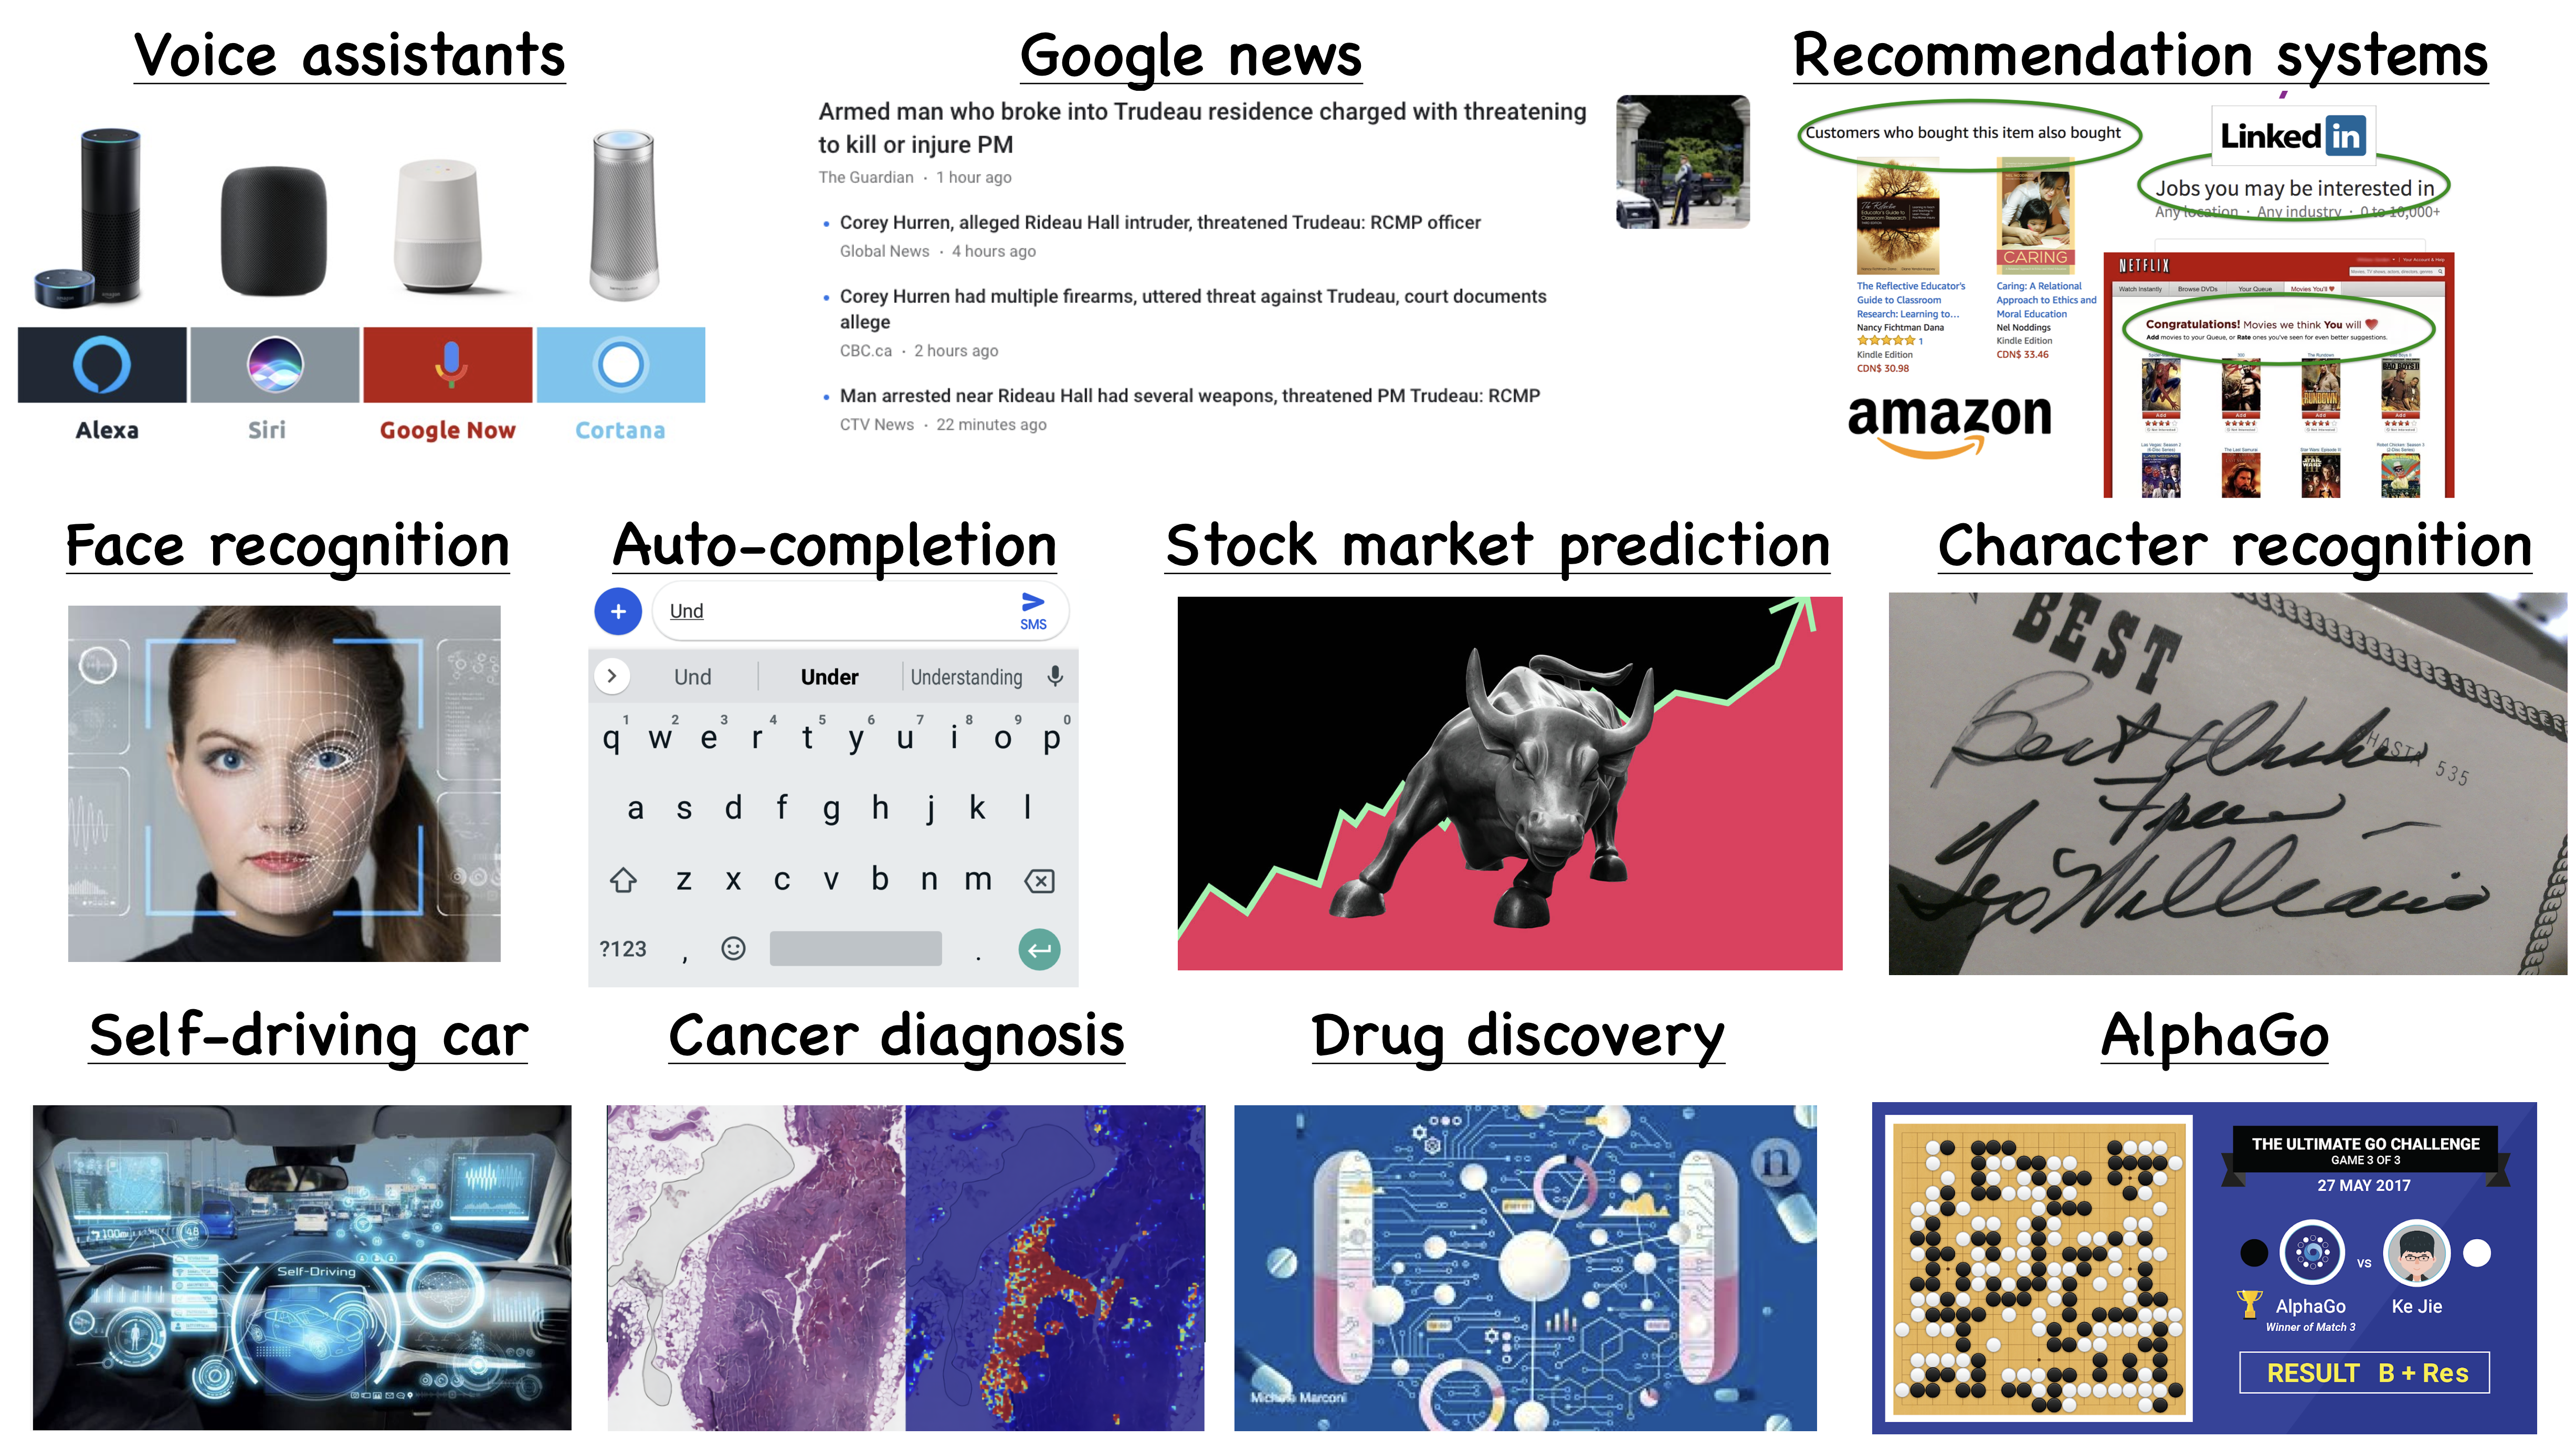
\includegraphics{/Users/charleenchu/Desktop/school/cpsc330-2023W2/lectures/img/ml-examples.png}

    \begin{itemize}
\tightlist
\item
  Image sources

  \begin{itemize}
  \tightlist
  \item
    \href{https://geeksfl.com/blog/best-voice-assistant/}{Voice
    assistants}
  \item
    \href{https://news.google.com}{Google News}\\
  \item
    \href{https://en.wikipedia.org/wiki/Recommender_system}{Recommendation
    systems}
  \item
    \href{https://startupleague.online/blog/3dss-tech-facial-recognition-technology/}{Face
    Recognition source}
  \item
    \href{https://9to5google.com/2020/08/10/android-11-autofill-keyboard/}{Auto-completion}
  \item
    \href{https://hbr.org/2019/12/what-machine-learning-will-mean-for-asset-managers}{Stock
    market prediction}\\
  \item
    \href{https://en.wikipedia.org/wiki/Handwriting_recognition}{Character
    recognition}\\
  \item
    \href{https://deepmind.com/alphago-china}{AlphaGo}
  \item
    \href{https://mc.ai/artificial-intelligence-in-self-driving-cars\%E2\%80\%8A-\%E2\%80\%8Ahow-far-have-we-gotten/}{Self-driving
    cars}
  \item
    \href{https://www.nature.com/articles/d41586-018-05267-x}{Drug
    discovery}
  \item
    \href{https://venturebeat.com/2018/10/12/google-ai-claims-99-accuracy-in-metastatic-breast-cancer-detection/}{Cancer
    detection}
  \end{itemize}
\end{itemize}

    \subsubsection{Saving time and scaling
products}\label{saving-time-and-scaling-products}

\begin{itemize}
\tightlist
\item
  Imagine writing a program for spam identification, i.e., whether an
  email is spam or non-spam.
\item
  Traditional programming

  \begin{itemize}
  \tightlist
  \item
    Come up with rules using human understanding of spam messages.
  \item
    Time consuming and hard to come up with robust set of rules.
  \end{itemize}
\item
  Machine learning

  \begin{itemize}
  \tightlist
  \item
    Collect large amount of data of spam and non-spam emails and let the
    machine learning algorithm figure out rules.
  \end{itemize}
\item
  With machine learning, you're likely to

  \begin{itemize}
  \tightlist
  \item
    Save time
  \item
    Customize and scale products
  \end{itemize}
\end{itemize}

    

    \subsection{Supervised machine
learning}\label{supervised-machine-learning}

    \subsubsection{Types of machine
learning}\label{types-of-machine-learning}

Here are some typical learning problems.

\begin{itemize}
\tightlist
\item
  \textbf{Supervised learning}
  (\href{https://support.google.com/a/answer/2368132?hl=en}{Gmail spam
  filtering})

  \begin{itemize}
  \tightlist
  \item
    Training a model from input data and its corresponding targets to
    predict targets for new examples.\\
  \end{itemize}
\item
  Unsupervised learning (\href{https://news.google.com/}{Google News})

  \begin{itemize}
  \tightlist
  \item
    Training a model to find patterns in a dataset, typically an
    unlabeled dataset.
  \end{itemize}
\item
  Reinforcement learning
  (\href{https://deepmind.com/research/case-studies/alphago-the-story-so-far}{AlphaGo})

  \begin{itemize}
  \tightlist
  \item
    A family of algorithms for finding suitable actions to take in a
    given situation in order to maximize a reward.
  \end{itemize}
\item
  Recommendation systems
  (\href{https://www.cs.umd.edu/~samir/498/Amazon-Recommendations.pdf}{Amazon
  item recommendation system})

  \begin{itemize}
  \tightlist
  \item
    Predict the ``rating'' or ``preference'' a user would give to an
    item.
  \end{itemize}
\end{itemize}

    \subsubsection{What is supervised machine learning
(ML)?}\label{what-is-supervised-machine-learning-ml}

\begin{itemize}
\tightlist
\item
  Training data comprises a set of observations (\(X\)) and their
  corresponding targets (\(y\)).
\item
  We wish to find a model function \(f\) that relates \(X\) to \(y\).
\item
  We use the model function to predict targets of new examples.
\end{itemize}

\includegraphics{/Users/charleenchu/Desktop/school/cpsc330-2023W2/lectures/img/sup-learning.png}

    \subsubsection{Example: Predict whether a message is spam or
not}\label{example-predict-whether-a-message-is-spam-or-not}

    \paragraph{\texorpdfstring{Input features \(X\) and target
\(y\)}{Input features X and target y}}\label{input-features-x-and-target-y}

    \texttt{\{note\}\ Do\ not\ worry\ about\ the\ code\ and\ syntax\ for\ now.}

    \texttt{\{note\}\ Download\ SMS\ Spam\ Collection\ Dataset\ from\ here:\ https://www.kaggle.com/uciml/sms-spam-collection-dataset.}

    \paragraph{\texorpdfstring{Training a supervised machine learning model
with \(X\) and
\(y\)}{Training a supervised machine learning model with X and y}}\label{training-a-supervised-machine-learning-model-with-x-and-y}

    \begin{tcolorbox}[breakable, size=fbox, boxrule=1pt, pad at break*=1mm,colback=cellbackground, colframe=cellborder]
\prompt{In}{incolor}{3}{\boxspacing}
\begin{Verbatim}[commandchars=\\\{\}]
\PY{n}{sms\PYZus{}df} \PY{o}{=} \PY{n}{pd}\PY{o}{.}\PY{n}{read\PYZus{}csv}\PY{p}{(}\PY{l+s+s2}{\PYZdq{}}\PY{l+s+s2}{data/spam.csv}\PY{l+s+s2}{\PYZdq{}}\PY{p}{,} \PY{n}{encoding}\PY{o}{=}\PY{l+s+s2}{\PYZdq{}}\PY{l+s+s2}{latin\PYZhy{}1}\PY{l+s+s2}{\PYZdq{}}\PY{p}{)}
\PY{n}{sms\PYZus{}df} \PY{o}{=} \PY{n}{sms\PYZus{}df}\PY{o}{.}\PY{n}{drop}\PY{p}{(}\PY{n}{columns} \PY{o}{=} \PY{p}{[}\PY{l+s+s2}{\PYZdq{}}\PY{l+s+s2}{Unnamed: 2}\PY{l+s+s2}{\PYZdq{}}\PY{p}{,} \PY{l+s+s2}{\PYZdq{}}\PY{l+s+s2}{Unnamed: 3}\PY{l+s+s2}{\PYZdq{}}\PY{p}{,} \PY{l+s+s2}{\PYZdq{}}\PY{l+s+s2}{Unnamed: 4}\PY{l+s+s2}{\PYZdq{}}\PY{p}{]}\PY{p}{)}
\PY{n}{sms\PYZus{}df} \PY{o}{=} \PY{n}{sms\PYZus{}df}\PY{o}{.}\PY{n}{rename}\PY{p}{(}\PY{n}{columns}\PY{o}{=}\PY{p}{\PYZob{}}\PY{l+s+s2}{\PYZdq{}}\PY{l+s+s2}{v1}\PY{l+s+s2}{\PYZdq{}}\PY{p}{:} \PY{l+s+s2}{\PYZdq{}}\PY{l+s+s2}{target}\PY{l+s+s2}{\PYZdq{}}\PY{p}{,} \PY{l+s+s2}{\PYZdq{}}\PY{l+s+s2}{v2}\PY{l+s+s2}{\PYZdq{}}\PY{p}{:} \PY{l+s+s2}{\PYZdq{}}\PY{l+s+s2}{sms}\PY{l+s+s2}{\PYZdq{}}\PY{p}{\PYZcb{}}\PY{p}{)}
\PY{n}{train\PYZus{}df}\PY{p}{,} \PY{n}{test\PYZus{}df} \PY{o}{=} \PY{n}{train\PYZus{}test\PYZus{}split}\PY{p}{(}\PY{n}{sms\PYZus{}df}\PY{p}{,} \PY{n}{test\PYZus{}size}\PY{o}{=}\PY{l+m+mf}{0.10}\PY{p}{,} \PY{n}{random\PYZus{}state}\PY{o}{=}\PY{l+m+mi}{42}\PY{p}{)}
\PY{n}{HTML}\PY{p}{(}\PY{n}{train\PYZus{}df}\PY{o}{.}\PY{n}{head}\PY{p}{(}\PY{p}{)}\PY{o}{.}\PY{n}{to\PYZus{}html}\PY{p}{(}\PY{n}{index}\PY{o}{=}\PY{k+kc}{False}\PY{p}{)}\PY{p}{)}
\end{Verbatim}
\end{tcolorbox}

            \begin{tcolorbox}[breakable, size=fbox, boxrule=.5pt, pad at break*=1mm, opacityfill=0]
\prompt{Out}{outcolor}{3}{\boxspacing}
\begin{Verbatim}[commandchars=\\\{\}]
<IPython.core.display.HTML object>
\end{Verbatim}
\end{tcolorbox}
        
    \begin{tcolorbox}[breakable, size=fbox, boxrule=1pt, pad at break*=1mm,colback=cellbackground, colframe=cellborder]
\prompt{In}{incolor}{4}{\boxspacing}
\begin{Verbatim}[commandchars=\\\{\}]
\PY{n}{X\PYZus{}train}\PY{p}{,} \PY{n}{y\PYZus{}train} \PY{o}{=} \PY{n}{train\PYZus{}df}\PY{p}{[}\PY{l+s+s2}{\PYZdq{}}\PY{l+s+s2}{sms}\PY{l+s+s2}{\PYZdq{}}\PY{p}{]}\PY{p}{,} \PY{n}{train\PYZus{}df}\PY{p}{[}\PY{l+s+s2}{\PYZdq{}}\PY{l+s+s2}{target}\PY{l+s+s2}{\PYZdq{}}\PY{p}{]}
\PY{n}{X\PYZus{}test}\PY{p}{,} \PY{n}{y\PYZus{}test} \PY{o}{=} \PY{n}{test\PYZus{}df}\PY{p}{[}\PY{l+s+s2}{\PYZdq{}}\PY{l+s+s2}{sms}\PY{l+s+s2}{\PYZdq{}}\PY{p}{]}\PY{p}{,} \PY{n}{test\PYZus{}df}\PY{p}{[}\PY{l+s+s2}{\PYZdq{}}\PY{l+s+s2}{target}\PY{l+s+s2}{\PYZdq{}}\PY{p}{]}
\PY{n}{clf} \PY{o}{=} \PY{n}{make\PYZus{}pipeline}\PY{p}{(}\PY{n}{CountVectorizer}\PY{p}{(}\PY{n}{max\PYZus{}features}\PY{o}{=}\PY{l+m+mi}{5000}\PY{p}{)}\PY{p}{,} \PY{n}{LogisticRegression}\PY{p}{(}\PY{n}{max\PYZus{}iter}\PY{o}{=}\PY{l+m+mi}{5000}\PY{p}{)}\PY{p}{)}
\PY{n}{clf}\PY{o}{.}\PY{n}{fit}\PY{p}{(}\PY{n}{X\PYZus{}train}\PY{p}{,} \PY{n}{y\PYZus{}train}\PY{p}{)}\PY{p}{;}
\end{Verbatim}
\end{tcolorbox}

    \paragraph{Predicting on unseen data using the trained
model}\label{predicting-on-unseen-data-using-the-trained-model}

    \begin{tcolorbox}[breakable, size=fbox, boxrule=1pt, pad at break*=1mm,colback=cellbackground, colframe=cellborder]
\prompt{In}{incolor}{5}{\boxspacing}
\begin{Verbatim}[commandchars=\\\{\}]
\PY{n}{pd}\PY{o}{.}\PY{n}{DataFrame}\PY{p}{(}\PY{n}{X\PYZus{}test}\PY{p}{[}\PY{l+m+mi}{0}\PY{p}{:}\PY{l+m+mi}{4}\PY{p}{]}\PY{p}{)}
\end{Verbatim}
\end{tcolorbox}

            \begin{tcolorbox}[breakable, size=fbox, boxrule=.5pt, pad at break*=1mm, opacityfill=0]
\prompt{Out}{outcolor}{5}{\boxspacing}
\begin{Verbatim}[commandchars=\\\{\}]
                                          sms
3245                                                  Funny fact Nobody teaches
volcanoes 2 erupt, tsunamis 2 arise, hurricanes 2 sway aroundn no 1 teaches hw 2
choose a wife Natural disasters just happens
944   I sent my scores to sophas and i had to do secondary application for a few
schools. I think if you are thinking of applying, do a research on cost also.
Contact joke ogunrinde, her school is one m{\ldots}
1044
We know someone who you know that fancies you. Call 09058097218 to find out who.
POBox 6, LS15HB 150p
2484
Only if you promise your getting out as SOON as you can. And you'll text me in
the morning to let me know you made it in ok.
\end{Verbatim}
\end{tcolorbox}
        
    \texttt{\{note\}\ Do\ not\ worry\ about\ the\ code\ and\ syntax\ for\ now.}

    \begin{tcolorbox}[breakable, size=fbox, boxrule=1pt, pad at break*=1mm,colback=cellbackground, colframe=cellborder]
\prompt{In}{incolor}{6}{\boxspacing}
\begin{Verbatim}[commandchars=\\\{\}]
\PY{n}{pred\PYZus{}dict} \PY{o}{=} \PY{p}{\PYZob{}}
    \PY{l+s+s2}{\PYZdq{}}\PY{l+s+s2}{sms}\PY{l+s+s2}{\PYZdq{}}\PY{p}{:} \PY{n}{X\PYZus{}test}\PY{p}{[}\PY{l+m+mi}{0}\PY{p}{:}\PY{l+m+mi}{4}\PY{p}{]}\PY{p}{,}
    \PY{l+s+s2}{\PYZdq{}}\PY{l+s+s2}{spam\PYZus{}predictions}\PY{l+s+s2}{\PYZdq{}}\PY{p}{:} \PY{n}{clf}\PY{o}{.}\PY{n}{predict}\PY{p}{(}\PY{n}{X\PYZus{}test}\PY{p}{[}\PY{l+m+mi}{0}\PY{p}{:}\PY{l+m+mi}{4}\PY{p}{]}\PY{p}{)}\PY{p}{,}
\PY{p}{\PYZcb{}}
\PY{n}{pred\PYZus{}df} \PY{o}{=} \PY{n}{pd}\PY{o}{.}\PY{n}{DataFrame}\PY{p}{(}\PY{n}{pred\PYZus{}dict}\PY{p}{)}
\PY{n}{pred\PYZus{}df}\PY{o}{.}\PY{n}{style}\PY{o}{.}\PY{n}{set\PYZus{}properties}\PY{p}{(}\PY{o}{*}\PY{o}{*}\PY{p}{\PYZob{}}\PY{l+s+s2}{\PYZdq{}}\PY{l+s+s2}{text\PYZhy{}align}\PY{l+s+s2}{\PYZdq{}}\PY{p}{:} \PY{l+s+s2}{\PYZdq{}}\PY{l+s+s2}{left}\PY{l+s+s2}{\PYZdq{}}\PY{p}{\PYZcb{}}\PY{p}{)}
\end{Verbatim}
\end{tcolorbox}

            \begin{tcolorbox}[breakable, size=fbox, boxrule=.5pt, pad at break*=1mm, opacityfill=0]
\prompt{Out}{outcolor}{6}{\boxspacing}
\begin{Verbatim}[commandchars=\\\{\}]
<pandas.io.formats.style.Styler at 0x10f102b30>
\end{Verbatim}
\end{tcolorbox}
        
    \textbf{We have accurately predicted labels for the unseen text messages
above!}

    

    \subsubsection{(Supervised) machine learning: popular
definition}\label{supervised-machine-learning-popular-definition}

A field of study that gives computers the ability to learn without being
explicitly programmed. -- Arthur Samuel (1959)

ML is a different way to think about problem solving.

\includegraphics{/Users/charleenchu/Desktop/school/cpsc330-2023W2/lectures/img/traditional-programming-vs-ML.png}

    \subsubsection{Examples}\label{examples}

Let's look at some concrete examples of supervised machine learning.

    \texttt{\{note\}\ Do\ not\ worry\ about\ the\ code\ at\ this\ point.\ Just\ focus\ on\ the\ input\ and\ output\ in\ each\ example.}

    \paragraph{Example 1: Predicting whether a patient has a liver disease
or
not}\label{example-1-predicting-whether-a-patient-has-a-liver-disease-or-not}

    \subparagraph{Input data}\label{input-data}

Suppose we are interested in predicting whether a patient has the
disease or not. We are given some tabular data with inputs and outputs
of liver patients, as shown below. The data contains a number of input
features and a special column called ``Target'' which is the output we
are interested in predicting.

    \texttt{\{note\}\ Download\ the\ data\ from\ https://www.kaggle.com/uciml/indian-liver-patient-records.}

    \begin{tcolorbox}[breakable, size=fbox, boxrule=1pt, pad at break*=1mm,colback=cellbackground, colframe=cellborder]
\prompt{In}{incolor}{7}{\boxspacing}
\begin{Verbatim}[commandchars=\\\{\}]
\PY{n}{df} \PY{o}{=} \PY{n}{pd}\PY{o}{.}\PY{n}{read\PYZus{}csv}\PY{p}{(}\PY{l+s+s2}{\PYZdq{}}\PY{l+s+s2}{data/indian\PYZus{}liver\PYZus{}patient.csv}\PY{l+s+s2}{\PYZdq{}}\PY{p}{)}
\PY{n}{df} \PY{o}{=} \PY{n}{df}\PY{o}{.}\PY{n}{drop}\PY{p}{(}\PY{n}{columns} \PY{o}{=} \PY{p}{[}\PY{l+s+s2}{\PYZdq{}}\PY{l+s+s2}{Gender}\PY{l+s+s2}{\PYZdq{}}\PY{p}{]}\PY{p}{)}
\PY{n}{df}\PY{p}{[}\PY{l+s+s2}{\PYZdq{}}\PY{l+s+s2}{Dataset}\PY{l+s+s2}{\PYZdq{}}\PY{p}{]} \PY{o}{=} \PY{n}{df}\PY{p}{[}\PY{l+s+s2}{\PYZdq{}}\PY{l+s+s2}{Dataset}\PY{l+s+s2}{\PYZdq{}}\PY{p}{]}\PY{o}{.}\PY{n}{replace}\PY{p}{(}\PY{l+m+mi}{1}\PY{p}{,} \PY{l+s+s2}{\PYZdq{}}\PY{l+s+s2}{Disease}\PY{l+s+s2}{\PYZdq{}}\PY{p}{)}
\PY{n}{df}\PY{p}{[}\PY{l+s+s2}{\PYZdq{}}\PY{l+s+s2}{Dataset}\PY{l+s+s2}{\PYZdq{}}\PY{p}{]} \PY{o}{=} \PY{n}{df}\PY{p}{[}\PY{l+s+s2}{\PYZdq{}}\PY{l+s+s2}{Dataset}\PY{l+s+s2}{\PYZdq{}}\PY{p}{]}\PY{o}{.}\PY{n}{replace}\PY{p}{(}\PY{l+m+mi}{2}\PY{p}{,} \PY{l+s+s2}{\PYZdq{}}\PY{l+s+s2}{No Disease}\PY{l+s+s2}{\PYZdq{}}\PY{p}{)}
\PY{n}{df}\PY{o}{.}\PY{n}{rename}\PY{p}{(}\PY{n}{columns}\PY{o}{=}\PY{p}{\PYZob{}}\PY{l+s+s2}{\PYZdq{}}\PY{l+s+s2}{Dataset}\PY{l+s+s2}{\PYZdq{}}\PY{p}{:} \PY{l+s+s2}{\PYZdq{}}\PY{l+s+s2}{Target}\PY{l+s+s2}{\PYZdq{}}\PY{p}{\PYZcb{}}\PY{p}{,} \PY{n}{inplace}\PY{o}{=}\PY{k+kc}{True}\PY{p}{)}
\PY{n}{train\PYZus{}df}\PY{p}{,} \PY{n}{test\PYZus{}df} \PY{o}{=} \PY{n}{train\PYZus{}test\PYZus{}split}\PY{p}{(}\PY{n}{df}\PY{p}{,} \PY{n}{test\PYZus{}size}\PY{o}{=}\PY{l+m+mi}{4}\PY{p}{,} \PY{n}{random\PYZus{}state}\PY{o}{=}\PY{l+m+mi}{42}\PY{p}{)}
\PY{n}{HTML}\PY{p}{(}\PY{n}{train\PYZus{}df}\PY{o}{.}\PY{n}{head}\PY{p}{(}\PY{p}{)}\PY{o}{.}\PY{n}{to\PYZus{}html}\PY{p}{(}\PY{n}{index}\PY{o}{=}\PY{k+kc}{False}\PY{p}{)}\PY{p}{)}
\end{Verbatim}
\end{tcolorbox}

            \begin{tcolorbox}[breakable, size=fbox, boxrule=.5pt, pad at break*=1mm, opacityfill=0]
\prompt{Out}{outcolor}{7}{\boxspacing}
\begin{Verbatim}[commandchars=\\\{\}]
<IPython.core.display.HTML object>
\end{Verbatim}
\end{tcolorbox}
        
    \subparagraph{Building a supervise machine learning
model}\label{building-a-supervise-machine-learning-model}

Let's train a supervised machine learning model with the input and
output above.

    

    \begin{tcolorbox}[breakable, size=fbox, boxrule=1pt, pad at break*=1mm,colback=cellbackground, colframe=cellborder]
\prompt{In}{incolor}{8}{\boxspacing}
\begin{Verbatim}[commandchars=\\\{\}]
\PY{k+kn}{from} \PY{n+nn}{lightgbm}\PY{n+nn}{.}\PY{n+nn}{sklearn} \PY{k+kn}{import} \PY{n}{LGBMClassifier}

\PY{n}{X\PYZus{}train} \PY{o}{=} \PY{n}{train\PYZus{}df}\PY{o}{.}\PY{n}{drop}\PY{p}{(}\PY{n}{columns}\PY{o}{=}\PY{p}{[}\PY{l+s+s2}{\PYZdq{}}\PY{l+s+s2}{Target}\PY{l+s+s2}{\PYZdq{}}\PY{p}{]}\PY{p}{)}
\PY{n}{y\PYZus{}train} \PY{o}{=} \PY{n}{train\PYZus{}df}\PY{p}{[}\PY{l+s+s2}{\PYZdq{}}\PY{l+s+s2}{Target}\PY{l+s+s2}{\PYZdq{}}\PY{p}{]}
\PY{n}{X\PYZus{}test} \PY{o}{=} \PY{n}{test\PYZus{}df}\PY{o}{.}\PY{n}{drop}\PY{p}{(}\PY{n}{columns}\PY{o}{=}\PY{p}{[}\PY{l+s+s2}{\PYZdq{}}\PY{l+s+s2}{Target}\PY{l+s+s2}{\PYZdq{}}\PY{p}{]}\PY{p}{)}
\PY{n}{y\PYZus{}test} \PY{o}{=} \PY{n}{test\PYZus{}df}\PY{p}{[}\PY{l+s+s2}{\PYZdq{}}\PY{l+s+s2}{Target}\PY{l+s+s2}{\PYZdq{}}\PY{p}{]}
\PY{n}{model} \PY{o}{=} \PY{n}{LGBMClassifier}\PY{p}{(}\PY{n}{random\PYZus{}state}\PY{o}{=}\PY{l+m+mi}{123}\PY{p}{,} \PY{n}{verbose}\PY{o}{=}\PY{o}{\PYZhy{}}\PY{l+m+mi}{1}\PY{p}{)}
\PY{n}{model}\PY{o}{.}\PY{n}{fit}\PY{p}{(}\PY{n}{X\PYZus{}train}\PY{p}{,} \PY{n}{y\PYZus{}train}\PY{p}{)}\PY{p}{;}
\end{Verbatim}
\end{tcolorbox}

    \subparagraph{Model predictions on unseen
data}\label{model-predictions-on-unseen-data}

\begin{itemize}
\tightlist
\item
  Given features of new patients below we'll use this model to predict
  whether these patients have the liver disease or not.
\end{itemize}

    \begin{tcolorbox}[breakable, size=fbox, boxrule=1pt, pad at break*=1mm,colback=cellbackground, colframe=cellborder]
\prompt{In}{incolor}{9}{\boxspacing}
\begin{Verbatim}[commandchars=\\\{\}]
\PY{n}{HTML}\PY{p}{(}\PY{n}{X\PYZus{}test}\PY{o}{.}\PY{n}{reset\PYZus{}index}\PY{p}{(}\PY{n}{drop}\PY{o}{=}\PY{k+kc}{True}\PY{p}{)}\PY{o}{.}\PY{n}{to\PYZus{}html}\PY{p}{(}\PY{n}{index}\PY{o}{=}\PY{k+kc}{False}\PY{p}{)}\PY{p}{)}
\end{Verbatim}
\end{tcolorbox}

            \begin{tcolorbox}[breakable, size=fbox, boxrule=.5pt, pad at break*=1mm, opacityfill=0]
\prompt{Out}{outcolor}{9}{\boxspacing}
\begin{Verbatim}[commandchars=\\\{\}]
<IPython.core.display.HTML object>
\end{Verbatim}
\end{tcolorbox}
        
    \begin{tcolorbox}[breakable, size=fbox, boxrule=1pt, pad at break*=1mm,colback=cellbackground, colframe=cellborder]
\prompt{In}{incolor}{10}{\boxspacing}
\begin{Verbatim}[commandchars=\\\{\}]
\PY{n}{pred\PYZus{}df} \PY{o}{=} \PY{n}{pd}\PY{o}{.}\PY{n}{DataFrame}\PY{p}{(}\PY{p}{\PYZob{}}\PY{l+s+s2}{\PYZdq{}}\PY{l+s+s2}{Predicted\PYZus{}target}\PY{l+s+s2}{\PYZdq{}}\PY{p}{:} \PY{n}{model}\PY{o}{.}\PY{n}{predict}\PY{p}{(}\PY{n}{X\PYZus{}test}\PY{p}{)}\PY{o}{.}\PY{n}{tolist}\PY{p}{(}\PY{p}{)}\PY{p}{\PYZcb{}}\PY{p}{)}

\PY{n}{df\PYZus{}concat} \PY{o}{=} \PY{n}{pd}\PY{o}{.}\PY{n}{concat}\PY{p}{(}\PY{p}{[}\PY{n}{pred\PYZus{}df}\PY{p}{,} \PY{n}{X\PYZus{}test}\PY{o}{.}\PY{n}{reset\PYZus{}index}\PY{p}{(}\PY{n}{drop}\PY{o}{=}\PY{k+kc}{True}\PY{p}{)}\PY{p}{]}\PY{p}{,} \PY{n}{axis}\PY{o}{=}\PY{l+m+mi}{1}\PY{p}{)}
\PY{n}{HTML}\PY{p}{(}\PY{n}{df\PYZus{}concat}\PY{o}{.}\PY{n}{to\PYZus{}html}\PY{p}{(}\PY{n}{index}\PY{o}{=}\PY{k+kc}{False}\PY{p}{)}\PY{p}{)}
\end{Verbatim}
\end{tcolorbox}

            \begin{tcolorbox}[breakable, size=fbox, boxrule=.5pt, pad at break*=1mm, opacityfill=0]
\prompt{Out}{outcolor}{10}{\boxspacing}
\begin{Verbatim}[commandchars=\\\{\}]
<IPython.core.display.HTML object>
\end{Verbatim}
\end{tcolorbox}
        
    

    \paragraph{Example 2: Predicting the label of a given
image}\label{example-2-predicting-the-label-of-a-given-image}

Suppose you want to predict the label of a given image using supervised
machine learning. We are using a pre-trained model here to predict
labels of new unseen images.

    ``\texttt{\{note\}\ Assuming\ that\ you\ have\ successfully\ created\ cpsc330}conda\texttt{environment\ on\ your\ computer,\ you\textquotesingle{}ll\ have\ to\ install}torchvision\texttt{in\ cpsc330}conda\texttt{environment\ to\ run\ the\ following\ code.\ If\ you\ are\ unable\ to\ install}torchvision`
on your laptop, please don't worry at this point. It's not crucial at
this point.

\begin{quote}
conda activate cpsc330 conda install -c pytorch torchvision ```
\end{quote}

    \begin{tcolorbox}[breakable, size=fbox, boxrule=1pt, pad at break*=1mm,colback=cellbackground, colframe=cellborder]
\prompt{In}{incolor}{11}{\boxspacing}
\begin{Verbatim}[commandchars=\\\{\}]
\PY{k+kn}{import} \PY{n+nn}{img\PYZus{}classify}
\PY{k+kn}{from} \PY{n+nn}{PIL} \PY{k+kn}{import} \PY{n}{Image}
\PY{k+kn}{import} \PY{n+nn}{glob}
\PY{k+kn}{import} \PY{n+nn}{matplotlib}\PY{n+nn}{.}\PY{n+nn}{pyplot} \PY{k}{as} \PY{n+nn}{plt}
\PY{c+c1}{\PYZsh{} Predict topn labels and their associated probabilities for unseen images}
\PY{n}{images} \PY{o}{=} \PY{n}{glob}\PY{o}{.}\PY{n}{glob}\PY{p}{(}\PY{l+s+s2}{\PYZdq{}}\PY{l+s+s2}{data/test\PYZus{}images/*.jpg}\PY{l+s+s2}{\PYZdq{}}\PY{p}{)}
\PY{n}{class\PYZus{}labels\PYZus{}file} \PY{o}{=} \PY{l+s+s1}{\PYZsq{}}\PY{l+s+s1}{data/imagenet\PYZus{}classes.txt}\PY{l+s+s1}{\PYZsq{}}
\PY{k}{for} \PY{n}{img\PYZus{}path} \PY{o+ow}{in} \PY{n}{images}\PY{p}{:}
    \PY{n}{img} \PY{o}{=} \PY{n}{Image}\PY{o}{.}\PY{n}{open}\PY{p}{(}\PY{n}{img\PYZus{}path}\PY{p}{)}\PY{o}{.}\PY{n}{convert}\PY{p}{(}\PY{l+s+s1}{\PYZsq{}}\PY{l+s+s1}{RGB}\PY{l+s+s1}{\PYZsq{}}\PY{p}{)}
    \PY{n}{img}\PY{o}{.}\PY{n}{load}\PY{p}{(}\PY{p}{)}
    \PY{n}{plt}\PY{o}{.}\PY{n}{imshow}\PY{p}{(}\PY{n}{img}\PY{p}{)}
    \PY{n}{plt}\PY{o}{.}\PY{n}{show}\PY{p}{(}\PY{p}{)}\PY{p}{;}    
    \PY{n}{df} \PY{o}{=} \PY{n}{img\PYZus{}classify}\PY{o}{.}\PY{n}{classify\PYZus{}image}\PY{p}{(}\PY{n}{img\PYZus{}path}\PY{p}{,} \PY{n}{class\PYZus{}labels\PYZus{}file}\PY{p}{)}
    \PY{n+nb}{print}\PY{p}{(}\PY{n}{df}\PY{o}{.}\PY{n}{to\PYZus{}string}\PY{p}{(}\PY{n}{index}\PY{o}{=}\PY{k+kc}{False}\PY{p}{)}\PY{p}{)}
    \PY{n+nb}{print}\PY{p}{(}\PY{l+s+s2}{\PYZdq{}}\PY{l+s+s2}{\PYZhy{}\PYZhy{}\PYZhy{}\PYZhy{}\PYZhy{}\PYZhy{}\PYZhy{}\PYZhy{}\PYZhy{}\PYZhy{}\PYZhy{}\PYZhy{}\PYZhy{}\PYZhy{}\PYZhy{}\PYZhy{}\PYZhy{}\PYZhy{}\PYZhy{}\PYZhy{}\PYZhy{}\PYZhy{}\PYZhy{}\PYZhy{}\PYZhy{}\PYZhy{}\PYZhy{}\PYZhy{}\PYZhy{}\PYZhy{}\PYZhy{}\PYZhy{}\PYZhy{}\PYZhy{}\PYZhy{}\PYZhy{}\PYZhy{}\PYZhy{}\PYZhy{}\PYZhy{}\PYZhy{}\PYZhy{}\PYZhy{}\PYZhy{}\PYZhy{}\PYZhy{}\PYZhy{}\PYZhy{}\PYZhy{}\PYZhy{}\PYZhy{}\PYZhy{}\PYZhy{}\PYZhy{}\PYZhy{}\PYZhy{}\PYZhy{}\PYZhy{}\PYZhy{}\PYZhy{}\PYZhy{}\PYZhy{}}\PY{l+s+s2}{\PYZdq{}}\PY{p}{)}
\end{Verbatim}
\end{tcolorbox}

    \begin{center}
    \adjustimage{max size={0.9\linewidth}{0.9\paperheight}}{output_50_0.png}
    \end{center}
    { \hspace*{\fill} \\}
    
    \begin{Verbatim}[commandchars=\\\{\}]
                                     Class  Probability score
         cheetah, chetah, Acinonyx jubatus              0.994
                  leopard, Panthera pardus              0.005
jaguar, panther, Panthera onca, Felis onca              0.001
       snow leopard, ounce, Panthera uncia              0.000
--------------------------------------------------------------
    \end{Verbatim}

    \begin{center}
    \adjustimage{max size={0.9\linewidth}{0.9\paperheight}}{output_50_2.png}
    \end{center}
    { \hspace*{\fill} \\}
    
    \begin{Verbatim}[commandchars=\\\{\}]
                         Class  Probability score
                     tiger cat              0.634
              tabby, tabby cat              0.177
Pembroke, Pembroke Welsh corgi              0.079
               lynx, catamount              0.011
--------------------------------------------------------------
    \end{Verbatim}

    \begin{center}
    \adjustimage{max size={0.9\linewidth}{0.9\paperheight}}{output_50_4.png}
    \end{center}
    { \hspace*{\fill} \\}
    
    \begin{Verbatim}[commandchars=\\\{\}]
                                   Class  Probability score
                                 macaque              0.885
patas, hussar monkey, Erythrocebus patas              0.062
      proboscis monkey, Nasalis larvatus              0.015
                       titi, titi monkey              0.010
--------------------------------------------------------------
    \end{Verbatim}

    \begin{center}
    \adjustimage{max size={0.9\linewidth}{0.9\paperheight}}{output_50_6.png}
    \end{center}
    { \hspace*{\fill} \\}
    
    \begin{Verbatim}[commandchars=\\\{\}]
                        Class  Probability score
Walker hound, Walker foxhound              0.570
             English foxhound              0.133
                  EntleBucher              0.074
                       beagle              0.065
--------------------------------------------------------------
    \end{Verbatim}

    

    \paragraph{Example 3: Predicting sentiment expressed in a movie
review}\label{example-3-predicting-sentiment-expressed-in-a-movie-review}

Suppose you are interested in predicting whether a given movie review is
positive or negative. You can do it using supervised machine learning.

    \texttt{\{note\}\ Download\ the\ data\ from\ https://www.kaggle.com/utathya/imdb-review-dataset.}

    \begin{tcolorbox}[breakable, size=fbox, boxrule=1pt, pad at break*=1mm,colback=cellbackground, colframe=cellborder]
\prompt{In}{incolor}{12}{\boxspacing}
\begin{Verbatim}[commandchars=\\\{\}]
\PY{n}{imdb\PYZus{}df} \PY{o}{=} \PY{n}{pd}\PY{o}{.}\PY{n}{read\PYZus{}csv}\PY{p}{(}\PY{l+s+s2}{\PYZdq{}}\PY{l+s+s2}{data/imdb\PYZus{}master.csv}\PY{l+s+s2}{\PYZdq{}}\PY{p}{,} \PY{n}{encoding}\PY{o}{=}\PY{l+s+s2}{\PYZdq{}}\PY{l+s+s2}{ISO\PYZhy{}8859\PYZhy{}1}\PY{l+s+s2}{\PYZdq{}}\PY{p}{)}
\PY{n}{imdb\PYZus{}df} \PY{o}{=} \PY{n}{imdb\PYZus{}df}\PY{p}{[}\PY{n}{imdb\PYZus{}df}\PY{p}{[}\PY{l+s+s2}{\PYZdq{}}\PY{l+s+s2}{label}\PY{l+s+s2}{\PYZdq{}}\PY{p}{]}\PY{o}{.}\PY{n}{str}\PY{o}{.}\PY{n}{startswith}\PY{p}{(}\PY{p}{(}\PY{l+s+s2}{\PYZdq{}}\PY{l+s+s2}{pos}\PY{l+s+s2}{\PYZdq{}}\PY{p}{,} \PY{l+s+s2}{\PYZdq{}}\PY{l+s+s2}{neg}\PY{l+s+s2}{\PYZdq{}}\PY{p}{)}\PY{p}{)}\PY{p}{]}
\PY{n}{imdb\PYZus{}df} \PY{o}{=} \PY{n}{imdb\PYZus{}df}\PY{o}{.}\PY{n}{drop}\PY{p}{(}\PY{n}{columns} \PY{o}{=} \PY{p}{[}\PY{l+s+s2}{\PYZdq{}}\PY{l+s+s2}{Unnamed: 0}\PY{l+s+s2}{\PYZdq{}}\PY{p}{,} \PY{l+s+s2}{\PYZdq{}}\PY{l+s+s2}{type}\PY{l+s+s2}{\PYZdq{}}\PY{p}{,} \PY{l+s+s2}{\PYZdq{}}\PY{l+s+s2}{file}\PY{l+s+s2}{\PYZdq{}}\PY{p}{]}\PY{p}{)}
\PY{n}{imdb\PYZus{}df}\PY{o}{.}\PY{n}{rename}\PY{p}{(}\PY{n}{columns}\PY{o}{=}\PY{p}{\PYZob{}}\PY{l+s+s2}{\PYZdq{}}\PY{l+s+s2}{label}\PY{l+s+s2}{\PYZdq{}}\PY{p}{:} \PY{l+s+s2}{\PYZdq{}}\PY{l+s+s2}{target}\PY{l+s+s2}{\PYZdq{}}\PY{p}{\PYZcb{}}\PY{p}{,} \PY{n}{inplace}\PY{o}{=}\PY{k+kc}{True}\PY{p}{)}
\PY{n}{train\PYZus{}df}\PY{p}{,} \PY{n}{test\PYZus{}df} \PY{o}{=} \PY{n}{train\PYZus{}test\PYZus{}split}\PY{p}{(}\PY{n}{imdb\PYZus{}df}\PY{p}{,} \PY{n}{test\PYZus{}size}\PY{o}{=}\PY{l+m+mf}{0.10}\PY{p}{,} \PY{n}{random\PYZus{}state}\PY{o}{=}\PY{l+m+mi}{123}\PY{p}{)}
\PY{n}{HTML}\PY{p}{(}\PY{n}{train\PYZus{}df}\PY{o}{.}\PY{n}{head}\PY{p}{(}\PY{p}{)}\PY{o}{.}\PY{n}{to\PYZus{}html}\PY{p}{(}\PY{n}{index}\PY{o}{=}\PY{k+kc}{False}\PY{p}{)}\PY{p}{)}
\end{Verbatim}
\end{tcolorbox}

            \begin{tcolorbox}[breakable, size=fbox, boxrule=.5pt, pad at break*=1mm, opacityfill=0]
\prompt{Out}{outcolor}{12}{\boxspacing}
\begin{Verbatim}[commandchars=\\\{\}]
<IPython.core.display.HTML object>
\end{Verbatim}
\end{tcolorbox}
        
    \begin{tcolorbox}[breakable, size=fbox, boxrule=1pt, pad at break*=1mm,colback=cellbackground, colframe=cellborder]
\prompt{In}{incolor}{13}{\boxspacing}
\begin{Verbatim}[commandchars=\\\{\}]
\PY{c+c1}{\PYZsh{} Build an ML model}
\PY{n}{X\PYZus{}train}\PY{p}{,} \PY{n}{y\PYZus{}train} \PY{o}{=} \PY{n}{train\PYZus{}df}\PY{p}{[}\PY{l+s+s2}{\PYZdq{}}\PY{l+s+s2}{review}\PY{l+s+s2}{\PYZdq{}}\PY{p}{]}\PY{p}{,} \PY{n}{train\PYZus{}df}\PY{p}{[}\PY{l+s+s2}{\PYZdq{}}\PY{l+s+s2}{target}\PY{l+s+s2}{\PYZdq{}}\PY{p}{]}
\PY{n}{X\PYZus{}test}\PY{p}{,} \PY{n}{y\PYZus{}test} \PY{o}{=} \PY{n}{test\PYZus{}df}\PY{p}{[}\PY{l+s+s2}{\PYZdq{}}\PY{l+s+s2}{review}\PY{l+s+s2}{\PYZdq{}}\PY{p}{]}\PY{p}{,} \PY{n}{test\PYZus{}df}\PY{p}{[}\PY{l+s+s2}{\PYZdq{}}\PY{l+s+s2}{target}\PY{l+s+s2}{\PYZdq{}}\PY{p}{]}

\PY{n}{clf} \PY{o}{=} \PY{n}{make\PYZus{}pipeline}\PY{p}{(}\PY{n}{CountVectorizer}\PY{p}{(}\PY{n}{max\PYZus{}features}\PY{o}{=}\PY{l+m+mi}{5000}\PY{p}{)}\PY{p}{,} \PY{n}{LogisticRegression}\PY{p}{(}\PY{n}{max\PYZus{}iter}\PY{o}{=}\PY{l+m+mi}{5000}\PY{p}{)}\PY{p}{)}
\PY{n}{clf}\PY{o}{.}\PY{n}{fit}\PY{p}{(}\PY{n}{X\PYZus{}train}\PY{p}{,} \PY{n}{y\PYZus{}train}\PY{p}{)}\PY{p}{;}
\end{Verbatim}
\end{tcolorbox}

    \begin{tcolorbox}[breakable, size=fbox, boxrule=1pt, pad at break*=1mm,colback=cellbackground, colframe=cellborder]
\prompt{In}{incolor}{14}{\boxspacing}
\begin{Verbatim}[commandchars=\\\{\}]
\PY{c+c1}{\PYZsh{} Predict on unseen data using the built model}
\PY{n}{pred\PYZus{}dict} \PY{o}{=} \PY{p}{\PYZob{}}
    \PY{l+s+s2}{\PYZdq{}}\PY{l+s+s2}{reviews}\PY{l+s+s2}{\PYZdq{}}\PY{p}{:} \PY{n}{X\PYZus{}test}\PY{p}{[}\PY{l+m+mi}{0}\PY{p}{:}\PY{l+m+mi}{4}\PY{p}{]}\PY{p}{,}
    \PY{l+s+s2}{\PYZdq{}}\PY{l+s+s2}{sentiment\PYZus{}predictions}\PY{l+s+s2}{\PYZdq{}}\PY{p}{:} \PY{n}{clf}\PY{o}{.}\PY{n}{predict}\PY{p}{(}\PY{n}{X\PYZus{}test}\PY{p}{[}\PY{l+m+mi}{0}\PY{p}{:}\PY{l+m+mi}{4}\PY{p}{]}\PY{p}{)}\PY{p}{,}
\PY{p}{\PYZcb{}}
\PY{n}{pred\PYZus{}df} \PY{o}{=} \PY{n}{pd}\PY{o}{.}\PY{n}{DataFrame}\PY{p}{(}\PY{n}{pred\PYZus{}dict}\PY{p}{)}
\PY{n}{pred\PYZus{}df}\PY{o}{.}\PY{n}{style}\PY{o}{.}\PY{n}{set\PYZus{}properties}\PY{p}{(}\PY{o}{*}\PY{o}{*}\PY{p}{\PYZob{}}\PY{l+s+s2}{\PYZdq{}}\PY{l+s+s2}{text\PYZhy{}align}\PY{l+s+s2}{\PYZdq{}}\PY{p}{:} \PY{l+s+s2}{\PYZdq{}}\PY{l+s+s2}{left}\PY{l+s+s2}{\PYZdq{}}\PY{p}{\PYZcb{}}\PY{p}{)}
\end{Verbatim}
\end{tcolorbox}

            \begin{tcolorbox}[breakable, size=fbox, boxrule=.5pt, pad at break*=1mm, opacityfill=0]
\prompt{Out}{outcolor}{14}{\boxspacing}
\begin{Verbatim}[commandchars=\\\{\}]
<pandas.io.formats.style.Styler at 0x10f102b90>
\end{Verbatim}
\end{tcolorbox}
        
    

    \paragraph{Example 4: Predicting housing
prices}\label{example-4-predicting-housing-prices}

Suppose we want to predict housing prices given a number of attributes
associated with houses.

    \texttt{\{note\}\ Download\ the\ data\ from\ https://www.kaggle.com/harlfoxem/housesalesprediction.}

    \begin{tcolorbox}[breakable, size=fbox, boxrule=1pt, pad at break*=1mm,colback=cellbackground, colframe=cellborder]
\prompt{In}{incolor}{15}{\boxspacing}
\begin{Verbatim}[commandchars=\\\{\}]
\PY{n}{df} \PY{o}{=} \PY{n}{pd}\PY{o}{.}\PY{n}{read\PYZus{}csv}\PY{p}{(}\PY{l+s+s2}{\PYZdq{}}\PY{l+s+s2}{data/kc\PYZus{}house\PYZus{}data.csv}\PY{l+s+s2}{\PYZdq{}}\PY{p}{)}
\PY{n}{df} \PY{o}{=} \PY{n}{df}\PY{o}{.}\PY{n}{drop}\PY{p}{(}\PY{n}{columns} \PY{o}{=} \PY{p}{[}\PY{l+s+s2}{\PYZdq{}}\PY{l+s+s2}{id}\PY{l+s+s2}{\PYZdq{}}\PY{p}{,} \PY{l+s+s2}{\PYZdq{}}\PY{l+s+s2}{date}\PY{l+s+s2}{\PYZdq{}}\PY{p}{]}\PY{p}{)}
\PY{n}{df}\PY{o}{.}\PY{n}{rename}\PY{p}{(}\PY{n}{columns}\PY{o}{=}\PY{p}{\PYZob{}}\PY{l+s+s2}{\PYZdq{}}\PY{l+s+s2}{price}\PY{l+s+s2}{\PYZdq{}}\PY{p}{:} \PY{l+s+s2}{\PYZdq{}}\PY{l+s+s2}{target}\PY{l+s+s2}{\PYZdq{}}\PY{p}{\PYZcb{}}\PY{p}{,} \PY{n}{inplace}\PY{o}{=}\PY{k+kc}{True}\PY{p}{)}
\PY{n}{train\PYZus{}df}\PY{p}{,} \PY{n}{test\PYZus{}df} \PY{o}{=} \PY{n}{train\PYZus{}test\PYZus{}split}\PY{p}{(}\PY{n}{df}\PY{p}{,} \PY{n}{test\PYZus{}size}\PY{o}{=}\PY{l+m+mf}{0.2}\PY{p}{,} \PY{n}{random\PYZus{}state}\PY{o}{=}\PY{l+m+mi}{4}\PY{p}{)}
\PY{n}{HTML}\PY{p}{(}\PY{n}{train\PYZus{}df}\PY{o}{.}\PY{n}{head}\PY{p}{(}\PY{p}{)}\PY{o}{.}\PY{n}{to\PYZus{}html}\PY{p}{(}\PY{n}{index}\PY{o}{=}\PY{k+kc}{False}\PY{p}{)}\PY{p}{)}
\end{Verbatim}
\end{tcolorbox}

            \begin{tcolorbox}[breakable, size=fbox, boxrule=.5pt, pad at break*=1mm, opacityfill=0]
\prompt{Out}{outcolor}{15}{\boxspacing}
\begin{Verbatim}[commandchars=\\\{\}]
<IPython.core.display.HTML object>
\end{Verbatim}
\end{tcolorbox}
        
    \begin{tcolorbox}[breakable, size=fbox, boxrule=1pt, pad at break*=1mm,colback=cellbackground, colframe=cellborder]
\prompt{In}{incolor}{16}{\boxspacing}
\begin{Verbatim}[commandchars=\\\{\}]
\PY{c+c1}{\PYZsh{} Build a regression model}
\PY{k+kn}{from} \PY{n+nn}{lightgbm}\PY{n+nn}{.}\PY{n+nn}{sklearn} \PY{k+kn}{import} \PY{n}{LGBMRegressor}

\PY{n}{X\PYZus{}train}\PY{p}{,} \PY{n}{y\PYZus{}train} \PY{o}{=} \PY{n}{train\PYZus{}df}\PY{o}{.}\PY{n}{drop}\PY{p}{(}\PY{n}{columns}\PY{o}{=} \PY{p}{[}\PY{l+s+s2}{\PYZdq{}}\PY{l+s+s2}{target}\PY{l+s+s2}{\PYZdq{}}\PY{p}{]}\PY{p}{)}\PY{p}{,} \PY{n}{train\PYZus{}df}\PY{p}{[}\PY{l+s+s2}{\PYZdq{}}\PY{l+s+s2}{target}\PY{l+s+s2}{\PYZdq{}}\PY{p}{]}
\PY{n}{X\PYZus{}test}\PY{p}{,} \PY{n}{y\PYZus{}test} \PY{o}{=} \PY{n}{test\PYZus{}df}\PY{o}{.}\PY{n}{drop}\PY{p}{(}\PY{n}{columns}\PY{o}{=} \PY{p}{[}\PY{l+s+s2}{\PYZdq{}}\PY{l+s+s2}{target}\PY{l+s+s2}{\PYZdq{}}\PY{p}{]}\PY{p}{)}\PY{p}{,} \PY{n}{train\PYZus{}df}\PY{p}{[}\PY{l+s+s2}{\PYZdq{}}\PY{l+s+s2}{target}\PY{l+s+s2}{\PYZdq{}}\PY{p}{]}

\PY{n}{model} \PY{o}{=} \PY{n}{LGBMRegressor}\PY{p}{(}\PY{n}{verbose}\PY{o}{=}\PY{o}{\PYZhy{}}\PY{l+m+mi}{1}\PY{p}{)}
\PY{n}{model}\PY{o}{.}\PY{n}{fit}\PY{p}{(}\PY{n}{X\PYZus{}train}\PY{p}{,} \PY{n}{y\PYZus{}train}\PY{p}{)}\PY{p}{;}
\end{Verbatim}
\end{tcolorbox}

    \begin{tcolorbox}[breakable, size=fbox, boxrule=1pt, pad at break*=1mm,colback=cellbackground, colframe=cellborder]
\prompt{In}{incolor}{17}{\boxspacing}
\begin{Verbatim}[commandchars=\\\{\}]
\PY{c+c1}{\PYZsh{} Predict on unseen examples using the built model}
\PY{n}{pred\PYZus{}df} \PY{o}{=} \PY{n}{pd}\PY{o}{.}\PY{n}{DataFrame}\PY{p}{(}
    \PY{c+c1}{\PYZsh{} \PYZob{}\PYZdq{}Predicted target\PYZdq{}: model.predict(X\PYZus{}test[0:4]).tolist(), \PYZdq{}Actual price\PYZdq{}: y\PYZus{}test[0:4].tolist()\PYZcb{}}
    \PY{p}{\PYZob{}}\PY{l+s+s2}{\PYZdq{}}\PY{l+s+s2}{Predicted\PYZus{}target}\PY{l+s+s2}{\PYZdq{}}\PY{p}{:} \PY{n}{model}\PY{o}{.}\PY{n}{predict}\PY{p}{(}\PY{n}{X\PYZus{}test}\PY{p}{[}\PY{l+m+mi}{0}\PY{p}{:}\PY{l+m+mi}{4}\PY{p}{]}\PY{p}{)}\PY{o}{.}\PY{n}{tolist}\PY{p}{(}\PY{p}{)}\PY{p}{\PYZcb{}}
\PY{p}{)}
\PY{n}{df\PYZus{}concat} \PY{o}{=} \PY{n}{pd}\PY{o}{.}\PY{n}{concat}\PY{p}{(}\PY{p}{[}\PY{n}{pred\PYZus{}df}\PY{p}{,} \PY{n}{X\PYZus{}test}\PY{p}{[}\PY{l+m+mi}{0}\PY{p}{:}\PY{l+m+mi}{4}\PY{p}{]}\PY{o}{.}\PY{n}{reset\PYZus{}index}\PY{p}{(}\PY{n}{drop}\PY{o}{=}\PY{k+kc}{True}\PY{p}{)}\PY{p}{]}\PY{p}{,} \PY{n}{axis}\PY{o}{=}\PY{l+m+mi}{1}\PY{p}{)}
\PY{n}{HTML}\PY{p}{(}\PY{n}{df\PYZus{}concat}\PY{o}{.}\PY{n}{to\PYZus{}html}\PY{p}{(}\PY{n}{index}\PY{o}{=}\PY{k+kc}{False}\PY{p}{)}\PY{p}{)}
\end{Verbatim}
\end{tcolorbox}

            \begin{tcolorbox}[breakable, size=fbox, boxrule=.5pt, pad at break*=1mm, opacityfill=0]
\prompt{Out}{outcolor}{17}{\boxspacing}
\begin{Verbatim}[commandchars=\\\{\}]
<IPython.core.display.HTML object>
\end{Verbatim}
\end{tcolorbox}
        
    To summarize, supervised machine learning can be used on a variety of
problems and different kinds of data.

    

    \subsubsection{🤔 Eva's questions}\label{evas-questions}

At this point, Eva is wondering about many questions.

\begin{itemize}
\tightlist
\item
  How are we exactly ``learning'' whether a message is spam and ham?
\item
  What do you mean by ``learn without being explicitly programmed''? The
  code has to be somewhere \ldots{}
\item
  Are we expected to get correct predictions for all possible messages?
  How does it predict the label for a message it has not seen before?\\
\item
  What if the model mis-labels an unseen example? For instance, what if
  the model incorrectly predicts a non-spam as a spam? What would be the
  consequences?
\item
  How do we measure the success or failure of spam identification?
\item
  If you want to use this model in the wild, how do you know how
  reliable it is?\\
\item
  Would it be useful to know how confident the model is about the
  predictions rather than just a yes or a no?
\end{itemize}

It's great to think about these questions right now. But Eva has to be
patient. By the end of this course you'll know answers to many of these
questions!

\includegraphics{/Users/charleenchu/Desktop/school/cpsc330-2023W2/lectures/img/eva-qm.png}

    \subsubsection{Machine learning
workflow}\label{machine-learning-workflow}

Supervised machine learning is quite flexible; it can be used on a
variety of problems and different kinds of data. Here is a typical
workflow of a supervised machine learning systems.

\includegraphics{/Users/charleenchu/Desktop/school/cpsc330-2023W2/lectures/img/ml-workflow.png}

We will build machine learning pipelines in this course, focusing on
some of the steps above.

    

    \subsubsection{❓❓ Questions for you}\label{questions-for-you}

\paragraph{iClicker join link:
https://join.iclicker.com/WMSX}\label{iclicker-join-link-httpsjoin.iclicker.comwmsx}

    \subsubsection{\texorpdfstring{Select all of the following statements
which are \textbf{True}
(iClicker)}{Select all of the following statements which are True (iClicker)}}\label{select-all-of-the-following-statements-which-are-true-iclicker}

\begin{itemize}
\tightlist
\item
  \begin{enumerate}
  \def\labelenumi{(\Alph{enumi})}
  \tightlist
  \item
    Predicting spam is an example of machine learning.
  \end{enumerate}
\item
  \begin{enumerate}
  \def\labelenumi{(\Alph{enumi})}
  \setcounter{enumi}{1}
  \tightlist
  \item
    Predicting housing prices is not an example of machine learning.
  \end{enumerate}
\item
  \begin{enumerate}
  \def\labelenumi{(\Alph{enumi})}
  \setcounter{enumi}{2}
  \tightlist
  \item
    For problems such as spelling correction, translation, face
    recognition, spam identification, if you are a domain expert, it's
    usually faster and scalable to come up with a robust set of rules
    manually rather than building a machine learning model.
  \end{enumerate}
\item
  \begin{enumerate}
  \def\labelenumi{(\Alph{enumi})}
  \setcounter{enumi}{3}
  \tightlist
  \item
    If you are asked to write a program to find all prime numbers up to
    a limit, it is better to implement one of the algorithms for doing
    so rather than using machine learning.
  \end{enumerate}
\item
  \begin{enumerate}
  \def\labelenumi{(\Alph{enumi})}
  \setcounter{enumi}{4}
  \tightlist
  \item
    Google News is likely using machine learning to organize news.
  \end{enumerate}
\end{itemize}

    

    

    \subsection{Break (5 min)}\label{break-5-min}

\includegraphics{/Users/charleenchu/Desktop/school/cpsc330-2023W2/lectures/img/eva-coffee.png}

\begin{itemize}
\tightlist
\item
  We will try to take a 5-minute break half way through every class.
\end{itemize}

    

    \subsection{About this course}\label{about-this-course}

    \subsubsection{Course website}\label{course-website}

    \begin{center}\rule{0.5\linewidth}{0.5pt}\end{center}

\url{https://github.com/UBC-CS/cpsc330-2023W2/} is the most important
link. Please read everything on this GitHub page! \_\_\_\_\_

    \begin{center}\rule{0.5\linewidth}{0.5pt}\end{center}

The \href{https://canvas.ubc.ca/courses/123439/quizzes}{Syllabus quiz}
is (will be) available on Canvas, Due: Monday, Jan 15th at 11:59pm.
\_\_\_\_\_

    \begin{center}\rule{0.5\linewidth}{0.5pt}\end{center}

The \href{}{first HomeWork} is (will be) available on Canvas, Due:
Monday, Jan 15th at 11:59pm. \_\_\_\_\_

    \subsubsection{CPSC 330 vs.~340}\label{cpsc-330-vs.-340}

Read
\url{https://github.com/UBC-CS/cpsc330-2023W1/blob/master/docs/330_vs_340.md}
which explains the difference between two courses.

\textbf{TLDR:}

\begin{itemize}
\tightlist
\item
  340: how do ML models work?
\item
  330: how do I use ML models?
\item
  CPSC 340 has many prerequisites.
\item
  CPSC 340 goes deeper but has a more narrow scope.
\item
  I think CPSC 330 will be more useful if you just plan to apply basic
  ML.
\end{itemize}

    \subsubsection{Registration, waitlist and
prerequisites}\label{registration-waitlist-and-prerequisites}

    \begin{center}\rule{0.5\linewidth}{0.5pt}\end{center}

Please go through
\href{https://github.com/UBC-CS/cpsc330-2023W2/blob/main/syllabus.md\#Registration}{this
document} carefully before contacting us (through the course email).
Even then, we are very unlikely to be able to help with registration,
waitlist or prerequisite issues. \_\_\_\_\_

    \subsubsection{Course format}\label{course-format}

\begin{itemize}
\tightlist
\item
  In person lectures T/Th at 9:30 am (Section 201) and T/Th at 3:30 pm
  (Section 202).
\item
  Sometimes there will be videos to watch before or during the lecture
  time. You will find the list of pre-watch videos on the course
  webpage.
\item
  First homework assignment is due \textbf{this coming Tuesday}, Sep
  12th, at 11:59pm. This is a relatively straightforward assignment on
  Python. If you struggle with this assignment then that could be a sign
  that you will struggle later on in the course.\\
\item
  You must do the first two homework assignments on your own.
\item
  I'm hoping you'll be able to work with partners on subsequent
  assignments pending the technology side of things.
\item
  Weekly tutorials will be \textbf{office hour format} run by the TAs
  and are \textbf{completely optional}.

  \begin{itemize}
  \tightlist
  \item
    You do not need to be registered in a tutorial.
  \item
    You can attend whatever tutorials or office hours your want,
    regardless of in which/whether you're registered.
  \end{itemize}
\item
  We'll have one midterm and one final.

  \begin{itemize}
  \tightlist
  \item
    Currently, we are thinking of closed-book Canvas exams.
  \end{itemize}
\end{itemize}

    \subsubsection{Course structure}\label{course-structure}

\begin{itemize}
\tightlist
\item
  Introduction

  \begin{itemize}
  \tightlist
  \item
    Week 1
  \end{itemize}
\item
  Part I: ML fundamentals and preprocessing

  \begin{itemize}
  \tightlist
  \item
    Weeks 2, 3, 4, 5, 6, 7, 8, midterm
  \end{itemize}
\item
  Part II: Unsupervised learning, transfer learning, common special
  cases

  \begin{itemize}
  \tightlist
  \item
    Weeks 9, 10, 11, 12
  \end{itemize}
\item
  Part III: Communication and ethics

  \begin{itemize}
  \tightlist
  \item
    ML skills are not beneficial if you can't use them responsibly and
    communicate your results. In this module we'll talk about these
    aspects.
  \item
    Weeks 13, 14
  \end{itemize}
\end{itemize}

    \subsubsection{Code of conduct}\label{code-of-conduct}

\begin{itemize}
\tightlist
\item
  Our main forum for getting help will be
  \href{https://piazza.com/class/lr4y28ceun367s}{Piazza}.
\end{itemize}

    Please read
\href{https://github.com/UBC-CS/cpsc330-2023W2//blob/master/docs/asking_for_help.md}{this
entire document about asking for help}.

\textbf{TL;DR:} Be nice.

    \subsubsection{Lecture and homework format: Jupyter
notebooks}\label{lecture-and-homework-format-jupyter-notebooks}

\begin{itemize}
\tightlist
\item
  This document is a \href{https://jupyter.org/}{Jupyter notebook}, with
  file extension \texttt{.ipynb}.
\item
  Confusingly, ``Jupyter notebook'' is also the original application
  that opens \texttt{.ipynb} files - but has since been replaced by
  \textbf{Jupyter lab}.

  \begin{itemize}
  \tightlist
  \item
    I am using Jupyter lab, some things might not work with the Jupyter
    notebook application.
  \item
    The course setup/install instructions include Jupyter lab.
  \end{itemize}
\item
  Jupyter notebooks contain a mix of code, code output,
  markdown-formatted text (including LaTeX equations), and more.

  \begin{itemize}
  \tightlist
  \item
    When you open a Jupyter notebook in one of these apps, the document
    is ``live'', meaning you can run the code.
  \item
    For example:
  \end{itemize}
\end{itemize}

    \begin{tcolorbox}[breakable, size=fbox, boxrule=1pt, pad at break*=1mm,colback=cellbackground, colframe=cellborder]
\prompt{In}{incolor}{17}{\boxspacing}
\begin{Verbatim}[commandchars=\\\{\}]
\PY{l+m+mi}{1} \PY{o}{+} \PY{l+m+mi}{1}
\end{Verbatim}
\end{tcolorbox}

            \begin{tcolorbox}[breakable, size=fbox, boxrule=.5pt, pad at break*=1mm, opacityfill=0]
\prompt{Out}{outcolor}{17}{\boxspacing}
\begin{Verbatim}[commandchars=\\\{\}]
2
\end{Verbatim}
\end{tcolorbox}
        
    \begin{tcolorbox}[breakable, size=fbox, boxrule=1pt, pad at break*=1mm,colback=cellbackground, colframe=cellborder]
\prompt{In}{incolor}{18}{\boxspacing}
\begin{Verbatim}[commandchars=\\\{\}]
\PY{n}{x} \PY{o}{=} \PY{p}{[}\PY{l+m+mi}{1}\PY{p}{,} \PY{l+m+mi}{2}\PY{p}{,} \PY{l+m+mi}{3}\PY{p}{]}
\PY{n}{x}\PY{p}{[}\PY{l+m+mi}{0}\PY{p}{]} \PY{o}{=} \PY{l+m+mi}{9999}
\PY{n}{x}
\end{Verbatim}
\end{tcolorbox}

            \begin{tcolorbox}[breakable, size=fbox, boxrule=.5pt, pad at break*=1mm, opacityfill=0]
\prompt{Out}{outcolor}{18}{\boxspacing}
\begin{Verbatim}[commandchars=\\\{\}]
[9999, 2, 3]
\end{Verbatim}
\end{tcolorbox}
        
    \begin{itemize}
\tightlist
\item
  By default, Jupyter prints out the result of the last line of code, so
  you don't need as many \texttt{print} statements.
\item
  In addition to the ``live'' notebooks, Jupyter notebooks can be
  statically rendered in the web browser,
  e.g.~\href{https://github.com/UBC-CS/cpsc330-2023W1/blob/master/lectures/01_intro.ipynb}{this}.

  \begin{itemize}
  \tightlist
  \item
    This can be convenient for quick read-only access, without needing
    to launch the Jupyter notebook/lab application.
  \item
    But you need to launch the app properly to interact with the
    notebooks.
  \end{itemize}
\end{itemize}

    \subsubsection{Lecture style}\label{lecture-style}

\begin{itemize}
\tightlist
\item
  Lots of code snippets in Jupyter.
\item
  There will be some
  \href{https://www.youtube.com/channel/UC40oUwJPrUmhsYdURk8OjqA}{YouTube
  videos} to watch before the lecture.
\item
  We will also try to work on some iClicker and Worksheets during the
  class.
\item
  All materials will be posted on the course website and
  \href{https://ubc-cs.github.io/cpsc330-2023W2}{this Jupyter book}.
\end{itemize}

    \paragraph{Lecture notes}\label{lecture-notes}

\begin{itemize}
\tightlist
\item
  All the lectures from last year are already
  \href{https://github.com/UBC-CS/cpsc330-2023W1}{available}.
\item
  I cannot promise anything will stay the same from last year to this
  year, so read them in advance at your own risk.
\item
  A ``finalized'' version will be pushed to
  \href{https://github.com/UBC-CS/cpsc330-2023W2/}{GitHub}.
\end{itemize}

    \subsubsection{Grades}\label{grades}

\begin{itemize}
\tightlist
\item
  The grading breakdown is
  \href{https://github.com/UBC-CS/cpsc330-2023W2/blob/main/syllabus.md\#Grading-scheme}{here}.
\item
  The policy on challenging grades is
  \href{https://github.com/UBC-CS/cpsc330-2023W2/blob/master/docs/grades.md}{here}.
\end{itemize}

    \subsection{Setting up your computer for the
course}\label{setting-up-your-computer-for-the-course}

    In this course, we will primarily be using Python, git, GitHub, Canvas,
Gradescope, and Piazza.

\begin{itemize}
\tightlist
\item
  Follow the setup instructions
  \href{https://github.com/UBC-CS/cpsc330-2023W2//blob/main/docs/setup.md}{here}
  to create a course \texttt{conda} environment on your computer.
\item
  If you do not have your computer with you, you can partner up with
  someone and set up your own computer later.
\end{itemize}

    \subsubsection{Python
requirements/resources}\label{python-requirementsresources}

We will primarily use Python in this course.

Here is the basic Python knowledge you'll need for the course:

\begin{itemize}
\tightlist
\item
  Basic Python programming
\item
  Numpy
\item
  Pandas
\item
  Basic matplotlib
\item
  Sparse matrices
\end{itemize}

Homework 1 is all about Python.

    \begin{center}\rule{0.5\linewidth}{0.5pt}\end{center}

\textbf{We do not have time to teach all the Python we need} but you can
find some useful Python resources
\href{https://github.com/UBC-CS/cpsc330-2023W1/blob/master/docs/resources.md}{here}.\\
\_\_\_\_\_

    

    \subsubsection{Checklist for you before the next
class}\label{checklist-for-you-before-the-next-class}

\begin{itemize}
\tightlist
\item[$\square$]
  Are you able to access course
  \href{https://canvas.ubc.ca/courses/130153}{Canvas}?
\item[$\square$]
  Are you able to access
  \href{https://piazza.com/class/lr4y28ceun367s}{course Piazza}?
\item[$\square$]
  Are you able to access \href{https://join.iclicker.com/WMSX}{iClicker}
  for this course?
\item[$\square$]
  Did you follow the setup instructions
  \href{https://github.com/UBC-CS/cpsc330-2023W2/blob/main/docs/setup.md}{here}
  to create a course conda environment on your computer?
\item[$\square$]
  Did you complete the syllabus quiz on Canvas?
\item[$\square$]
  Are you almost finished or at least started with homework 1?
\end{itemize}

    

    

    \subsection{Summary}\label{summary}

\begin{itemize}
\tightlist
\item
  Machine learning is a different paradigm for problem solving.\\
\item
  Very often it reduces the time you spend programming and helps
  customizing and scaling your products.
\item
  In supervised learning we are given a set of observations (\(X\)) and
  their corresponding targets (\(y\)) and we wish to find a model
  function \(f\) that relates \(X\) to \(y\).
\item
  Carefully read the course website. Make sure to complete the surveys.
\item
  \textbf{The teaching team is here to help you learn the material and
  succeed in the course!}
\item
  This semester can be particularly difficult with in-person transition
  after the pandemic. Please reach out if you are going through hard
  time. I'll try my best to be accommodative and empathetic.
\item
  Let's have fun learning this material together!
\end{itemize}

    \includegraphics{/Users/charleenchu/Desktop/school/cpsc330-2023W2/lectures/img/eva-seeyou.png}


    % Add a bibliography block to the postdoc
    
    
    
\end{document}
